\documentclass[a4paper,fleqn]{cas-dc}

\usepackage[numbers,sort&compress]{natbib}
\usepackage{amsmath,amssymb,amsfonts}
\usepackage{graphicx}
\usepackage{booktabs}
\usepackage{multirow}
\usepackage{xcolor}
\usepackage{hyperref}
\usepackage{listings}
\usepackage{subcaption}
\usepackage{array}
\usepackage{tabularx}
\usepackage{amsthm}

\newtheorem{proposition}{Proposition}

% Relax LaTeX float placement restrictions so figures stay in their sections
\renewcommand{\topfraction}{0.95}
\renewcommand{\bottomfraction}{0.85}
\setcounter{topnumber}{4}
\setcounter{bottomnumber}{3}
\setcounter{totalnumber}{8}
\setcounter{dbltopnumber}{4}
\renewcommand{\dbltopfraction}{0.95}
\renewcommand{\textfraction}{0.05}
\renewcommand{\floatpagefraction}{0.65}
\renewcommand{\dblfloatpagefraction}{0.65}

% Custom macros for exact empirical constants from the frozen Number Bank
% (paper/CEA Paper/manuscript/NUMBER_BANK.md -- every value below traces there).
\newcommand{\Nmisbind}{10{,}000}
\newcommand{\Nslots}{11}
\newcommand{\MisbindDetRate}{100.0\%}
\newcommand{\DetAdvisoryCoverage}{51.04\%}
\newcommand{\SafetyRefusalHandling}{10.48\%}
\newcommand{\LLMDependent}{38.48\%}
\newcommand{\LatencySpeedup}{2.28\times}
\newcommand{\SearchSpaceRedPct}{75.64\%}
\newcommand{\DialectHitAdvantage}{+36.6\,\text{pp}}
\newcommand{\SMSFidelity}{100.0\%}
\newcommand{\SMSHazardLLM}{64.4\%}
\newcommand{\TamperDetRate}{100.0\%}

\begin{document}
\let\WriteBookmarks\relax

% Short title and author running heads
\shorttitle{Neurosymbolic Safeguards for Agricultural Advisory}
\shortauthors{K. R. I. Reza et~al.}

\title [mode = title]{Neurosymbolic Safeguards for Agricultural Advisory: Deterministic Contract Verification in Safety-Critical Crop Protection}

\author[1]{Khan Raiyan Ibne Reza}[type=editor,auid=000,bioid=1,orcid=0009-0002-8610-8673]
\cormark[1]
\ead{raiyan.reza@northsouth.edu}
\credit{Conceptualization, Methodology, Software, Formal Analysis, Writing - Original Draft, Writing - Review \& Editing}

\author[1]{Sanjana Aktar Maria}
\ead{sanjana.maria@northsouth.edu}
\credit{Investigation, Data Curation, Validation, Writing - Review \& Editing}

\author[1]{Shakil Ahmed}
\ead{shakil.ahmed02@northsouth.edu}
\credit{Software, Resources, Investigation}

\author[1]{Sumaiya Tabassum Nimi}
\ead{sumaiya.nimi@northsouth.edu}
\credit{Data Curation, Validation, Formal Analysis}

\address[1]{Department of Computer Science and Engineering, North South University, Dhaka 1229, Bangladesh}

\cortext[1]{Corresponding author}

\begin{abstract}
Pesticide recommendations are safety-critical: a single misbinding between a valid active ingredient and an incorrect dosage or pre-harvest interval can cause poisoning or environmental harm. We present \textbf{KrishokChat}, a neurosymbolic agricultural advisory system that separates factual authority from generative language through an 11-slot, single-record, fail-closed deterministic certification contract. A claim is certified only when all 11 contract fields are jointly satisfied by one accredited evidence record; failure triggers deterministic abstention or escalation.

We evaluate the certification contract exhaustively across all 11 mutation classes and 40 base agronomic records (440 coverage cells). The certification predicate rejected every case in every cell. Controlled ablation against an 8-slot contract (B5) demonstrates that slot completeness accounts for the corresponding corruption vulnerabilities. Empirical slot ablation (crop validation yielding an 8.94\,pp hazard surge and provenance hash integrity yielding 8.92\,pp when removed) and a benign-mutation control (0.0\% false rejection on approved actives, 3.67\% on restricted chemicals) confirm that the predicate is both necessary and discriminating.

On a 100-case live end-to-end benchmark, KrishokChat achieves 83.0\% certified advisory correctness with 1.0\% critical unsafe acceptance (versus 8.0\% for direct LLMs and 15.0\% for LLM-as-a-judge guardrails). Under temporal and cross-modal conflicts, KrishokChat eliminates hazardous recommendations (0.0\% critical unsafe acceptance versus 39.0\%--75.0\% for baseline models and post-hoc judges). The architecture is evaluated on an institutional crop-protection corpus from BARI, BRRI, and DAE/MoA. All benchmark datasets, verification code, and models are released under open licenses.
\end{abstract}

\begin{keywords}
Agricultural decision support \sep Neurosymbolic AI \sep Large language models \sep Retrieval-augmented generation \sep Safety-critical verification \sep Deterministic contract verification \sep Selective resolution \sep Edge computing
\end{keywords}

\maketitle

% =========================================================================
% Section Source: sections/01_introduction.tex
% =========================================================================
% Section 1: Introduction — revised per CEA editorial review
\section{Introduction}
\label{sec:introduction}

\subsection{Agricultural Advisory Is an Action-Authorization Problem}
Large language models (LLMs) are becoming a practical interface for agricultural advisory because they allow farmers to describe problems in ordinary language rather than navigate technical manuals, decision trees, or specialized software. Systems such as Farmer.Chat have demonstrated the feasibility of LLM-based advisory for smallholder farmers, while recent agricultural research has extended this paradigm with retrieval-augmented generation (RAG), structured knowledge, temporal retrieval, and multimodal diagnosis \citep{farmerchat2024,goatrag2026,tarag2026,smart2026}. In Bangladesh, KrishokBondhu has further shown that retrieval-augmented conversational assistance can be delivered directly to Bengali-speaking farmers through a voice-based interface \citep{krishokbondhu2025}.

The central difficulty is that crop-protection advice is not an ordinary question-answering task. A recommendation to apply a pesticide is an actionable decision whose safety depends on several variables being simultaneously correct: the target crop, pest or disease, crop stage, active ingredient, formulation, dosage range, measurement unit, water-volume denominator, spray interval, and pre-harvest interval (PHI). Regulatory status is an additional constraint because a recommendation that was valid in an earlier period may become restricted or prohibited later. An error in any one of these fields can turn an otherwise plausible recommendation into an inappropriate treatment, excessive application, or use of a compound that is no longer authorized.

This makes the problem fundamentally different from conventional factual question answering. The system must not merely produce statements that are individually supported by retrieved documents; it must ensure that the \emph{actionable combination} is valid. For example, a retrieval system may find a valid pesticide for one crop, a valid dosage from another entry, and a valid PHI from a third. Each statement may be genuine, yet their combination may not correspond to any approved treatment. In such a setting, fluency and even document-level grounding are insufficient indicators of safety.

\subsection{The Difficulty Begins Before Generation}
The problem is further complicated by the way farmers actually ask questions. Agricultural queries are often incomplete, colloquial, context-dependent, or expressed in forms that differ substantially from the terminology used in extension manuals. In Bangladesh, the same intent may appear in formal Bengali, everyday farmer language, regional varieties such as Sylheti or Chittagonian, or Romanized Banglish. Farmers may also omit critical information, switch crops during a conversation, describe symptoms without naming the crop, or state a treatment assumption as if it were already confirmed.

For standard information retrieval, such colloquial and incomplete inputs primarily degrade relevance. In crop-protection advisory, however, they introduce critical safety hazards. For instance, in an underspecified query such as \emph{``Patay dag hoyeche, ki spray korbo?''} (``Spots on leaves; what to spray?''), omitting the crop prevents the system from identifying valid disease and treatment relationships. An unconstrained generative model that silently assumes a crop converts linguistic ambiguity into hazardous chemical advice. Conversely, indiscriminately rejecting every incomplete query renders the system unhelpful.

Recent agricultural systems have begun to address individual parts of this problem. TARAG incorporates temporal information into agricultural retrieval so that recommendations remain aligned with crop and pest timelines \citep{tarag2026}; SMART combines structured semantics, retrieval, multimodal evidence, and human verification for plant-disease diagnosis \citep{smart2026}; and Bengali agricultural advisory systems have demonstrated the importance of adapting retrieval and interaction to local users \citep{krishokbondhu2025}. These advances make agricultural AI more capable, but they do not remove the underlying authority problem: better retrieval or better perception does not by itself determine whether a complete safety-critical action is authorized.

\subsection{Why Retrieval and Generation Alone Are Not Enough}
The broader RAG literature has increasingly recognized that retrieving evidence is not equivalent to producing a faithful answer. RAGChecker introduced fine-grained diagnosis of retrieval and generation failures, while subsequent work has investigated explicit verification of generated answers, fact-level conflicts, provenance, and adversarial manipulation of retrieved evidence \citep{ragchecker2024,generateverify2025,faithfulrag2025,saferag2025}. These studies show that a system can fail even when relevant evidence is present: the generator may omit a critical fact, introduce a conflicting prior, or combine pieces of evidence in a way that is not justified by any single source.

Agricultural advisory makes this problem particularly consequential because the relevant facts are relational. The question is not simply whether a generated dosage appears somewhere in the evidence. The relevant dosage must belong to the correct crop--problem--formulation context and must remain compatible with the other safety-critical attributes of the same recommendation. Temporal changes create another source of inconsistency: an older institutional document may contain a genuine recommendation that is no longer valid under a later regulatory decision. Thus, retrieval relevance, citation presence, and textual faithfulness are necessary signals, but they are not sufficient authorization criteria for an actionable pesticide recommendation.

This motivates a different design principle for safety-critical agricultural AI:
\begin{quote}
\emph{The component that generates fluent language should not be the component that holds factual authority for safety-critical actions.}
\end{quote}
The principle separates two responsibilities that are often conflated in conversational systems. Neural models remain useful for language understanding, perception, retrieval, explanation, and natural-language realization. Factual authority, however, is assigned to a structured evidence layer whose conditions can be checked deterministically before an action is released.

\subsection{KrishokChat: Bounded Authority Through Deterministic Certification}
We present \textbf{KrishokChat}, an advisory framework designed around this separation of authority. The architecture represents crop-protection advice as an 11-slot decision contract comprising the crop, problem, growth stage, active ingredient, formulation, dosage bounds, unit, water-volume denominator, spray interval, and PHI. These semantic fields are paired with an evidence-governance layer containing source authority, regulatory status, temporal validity, version information, and provenance.

The key restriction is applied at runtime. A safety-critical recommendation is not certified merely because each field can be found somewhere in the retrieved context. The complete tuple must be jointly supported by one canonical, provenance-traceable authority record that is valid for the current regulatory state. Multi-source institutional knowledge can still be reconciled during controlled knowledge compilation, but runtime generation is prohibited from freely recombining safety-critical fields across records. When the required conditions are not satisfied, the system does not attempt to repair the missing evidence through further free-form generation. It instead transitions to a bounded alternative: deterministic resolution, clarification, safe non-chemical guidance, abstention, or escalation.

This authority boundary also determines how uncertainty is handled throughout the system. A lightweight language router may misinterpret a farmer's wording; an image model may be uncertain about crop identity; retrieval may return an incomplete or conflicting record; regulations may have changed; or the knowledge base may simply lack the required evidence. None of these components is allowed to convert its uncertainty directly into a chemical action. Instead, uncertainty reduces the system's authority and triggers a controlled response. In this sense, clarification, abstention, and fallback guidance are not merely interface behaviors: they are mechanisms for preventing uncertainty from propagating into unsafe recommendations.

The resulting architecture separates three concerns that are typically collapsed into one generative step. First, the system interprets the farmer's language and available context. Second, it resolves candidate agricultural evidence under explicit authority and validity rules. Third, it permits generation only within the boundary established by the certified evidence. The same boundary is maintained when the interaction is multilingual or dialectal, spans multiple turns, contains conflicting image and text evidence, encounters adversarial input, or operates under constrained connectivity.

\subsection{Research Questions and Contributions}
The central research question is whether explicitly separating factual authority from generative language can improve the reliability of agricultural LLM advisory without reducing the system to a universally conservative refusal mechanism. We investigate this question across five dimensions: advisory correctness, relational safety, uncertainty handling, robustness to changing and adversarial conditions, and constrained deployment.

The contributions of this work are threefold:
\begin{enumerate}
\item \textbf{A bounded-authority certification mechanism for safety-critical agricultural advice.} We introduce an 11-slot relational contract in which a pesticide recommendation can be certified only when its safety-critical attributes are complete, jointly consistent, current, and traceable to a canonical authority record. This design specifically targets cross-record relational misbinding, in which individually valid agricultural facts are combined into an unauthorized action.
\item \textbf{An uncertainty-preserving selective resolution policy.} We formulate a resolution framework distinguishing deterministic certification, bounded realization, targeted clarification, non-chemical agronomic guidance, abstention, and human escalation. This architecture allows the system to assist farmers even when queries are underspecified, dialectal, or contradictory, without empowering the language model to synthesize unverified safety-critical parameters.
\item \textbf{A multi-axis evaluation of reliability under realistic agricultural failure modes.} We evaluate the architecture using controlled relational corruption, retrieval failures, temporal regulatory conflicts, adversarial inputs, Bengali linguistic variation, confused and underspecified farmer queries, multi-turn pressure, multimodal disagreement, knowledge-base incompleteness, and constrained deployment conditions. The evaluation is designed to test not only whether the system produces good answers, but whether unsafe actions remain outside the system's certified output space when upstream components are uncertain or incorrect.
\end{enumerate}

This perspective is deliberately narrower than claiming that agricultural LLMs can be made ``hallucination-free.'' Instead, the objective is to make a precise class of high-consequence actions subject to an explicit authority condition. The language model remains valuable as a conversational interface, but the authority to release a safety-critical agricultural action resides outside the generator and is granted only after deterministic verification.

The remainder of this paper is organized as follows. Section~\ref{sec:related_work} positions the work against the literature. Section~\ref{sec:problem_formulation} formalizes the problem and the certification contract. Section~\ref{sec:system_architecture} describes the architecture, and Section~\ref{sec:knowledge_governance} details knowledge governance. Section~\ref{sec:experimental_methodology} presents the methodology. Sections~\ref{sec:results_advisory_quality}--\ref{sec:results_deployment} report results organized by research question. Sections~\ref{sec:discussion}--\ref{sec:conclusion} present the discussion, deployment implications, limitations, data and code availability, and conclusion.
% =========================================================================
% Section 2: Related Work
% =========================================================================
\section{Related Work}
\label{sec:related_work}

Table~\ref{tab:literature_positioning} provides a systematic positioning of the present work against representative systems across agricultural conversational AI, structured knowledge systems, and selective prediction. The comparison reveals that while individual properties---multilingual fluency, structured facts, temporal awareness, multimodal conditioning, offline operation, and fail-closed safety---have each been demonstrated in isolation, no evaluated system binds a safety-critical advisory contract to a single authoritative record and selectively resolves across deterministic, generative, and abstention paths.


% =========================================================================
% Inlined Table: tables/tab2_literature_positioning.tex
% =========================================================================
\begin{table*}[pos=t]
\centering
\caption{Systematic positioning of KrishokChat alongside contemporary agricultural AI, retrieval-augmented decision support, and low-resource advisory systems.}
\label{tab:literature_positioning}
\small
\resizebox{\textwidth}{!}{\begin{tabular}{lcccccccc}
\toprule
\textbf{System / Framework} & \textbf{Language} & \textbf{Domain} & \textbf{RAG} & \textbf{Structured Facts} & \textbf{Temporal} & \textbf{Multimodal} & \textbf{Fail-Closed} & \textbf{Edge/Offline} \\
\midrule
Farmer.Chat \citep{farmerchat2024} & Multilingual & General Agri & \checkmark & Partial & $\times$ & $\times$ & $\times$ & $\times$ \\
KrishokBondhu \citep{krishokbondhu2025} & Bengali & Crop Advisory & \checkmark & $\times$ & $\times$ & Voice & $\times$ & $\times$ \\
Domain-First RAG \citep{goatrag2026} & German/English & Livestock & \checkmark & \checkmark & $\times$ & $\times$ & $\times$ & $\times$ \\
TARAG \citep{tarag2026} & Chinese/English & Crop Diseases & \checkmark & $\times$ & \checkmark & $\times$ & $\times$ & $\times$ \\
SMART \citep{smart2026} & English/Hindi & Plant Pathology & \checkmark & \checkmark & $\times$ & \checkmark & HITL & $\times$ \\
AgroTutor \citep{agrotutor2020} & Spanish & Crop Planning & $\times$ & \checkmark & $\times$ & $\times$ & $\times$ & \checkmark \\
\textbf{KrishokChat (This Work)} & \textbf{Bengali} & \textbf{Crop Advisory} & \textbf{\checkmark} & \textbf{\checkmark} & \textbf{\checkmark} & \textbf{\checkmark} & \textbf{\checkmark} & \textbf{\checkmark} \\
\bottomrule
\end{tabular}}
\end{table*}
% =========================================================================


\subsection{Agricultural Conversational AI and Retrieval-Augmented Advisory}
Large language models have recently become a practical interface for agricultural decision support, particularly when combined with retrieval from domain-specific knowledge bases. Farmer.Chat demonstrated the feasibility of scaling multilingual AI-powered agricultural services for smallholder farmers, establishing a conversational alternative to conventional extension interfaces \citep{farmerchat2024}. In Bangladesh, KrishokBondhu extended this direction to Bengali-speaking farmers through a voice-enabled, retrieval-augmented call-center system that combines agricultural documents, Bengali speech processing, semantic retrieval, and LLM-based response generation \citep{krishokbondhu2025}. These systems establish the usefulness of generative interfaces for agricultural knowledge access, but their primary objective is to improve accessibility and answer quality rather than to make the release of safety-critical actions subject to a formal authorization condition.

Recent work has substantially broadened the capabilities of agricultural RAG. Domain-specific systems have incorporated structured decision knowledge into retrieval pipelines for livestock advisory, while DSSAT-LM connects language models to crop simulation so that free-form questions can be translated into structured agricultural decision variables \citep{goatrag2026,dssatlm2026}. TARAG introduces temporal knowledge representation and time-aware re-ranking for crop pest and disease management, explicitly recognizing that agricultural recommendations depend on changing phenology, pest life cycles, and temporal context \citep{tarag2026}. SMART combines structured semantics, retrieval, multimodal evidence, and human-in-the-loop verification for plant disease diagnosis, addressing robustness to noisy inputs and long-tailed visual classes \citep{smart2026}. Lightweight and offline agricultural decision-support systems have also been studied, including mobile advisory systems designed for data-scarce environments \citep{agrotutor2020}.

This progression is important for the positioning of the present work. The challenge is no longer simply to retrieve agricultural information, add a domain knowledge base, or place an LLM behind a farmer-facing interface. Contemporary agricultural systems already address temporal retrieval, structured knowledge, multimodal diagnosis, and deployment constraints. The remaining question for safety-critical crop protection is more specific: \emph{when a system produces an actionable recommendation, what mechanism determines that the complete recommendation is authorized rather than merely plausible?}

\subsection{RAG Faithfulness, Provenance, and Security}
The broader RAG literature has increasingly demonstrated that retrieval does not guarantee faithful generation. RAGChecker introduced fine-grained diagnosis of retrieval and generation failures, separating problems in evidence retrieval from failures in the generated response \citep{ragchecker2024}. Generate but Verify subsequently formulated faithfulness assessment as an explicit downstream task and showed that better faithfulness prediction can improve the behavior of RAG applications \citep{generateverify2025}. Fact-level approaches have also investigated situations in which retrieved evidence conflicts with the language model's parametric knowledge; FaithfulRAG, for example, explicitly models conflicts between retrieved and parametric facts rather than treating retrieved context as automatically authoritative \citep{faithfulrag2025}. Provenance-oriented methods similarly aim to trace unsupported generated claims back to their evidential context, providing low-latency mechanisms for identifying factual errors in RAG outputs \citep{scifact2020}.

Security research further challenges the assumption that retrieved evidence can be trusted simply because it came from the retrieval layer. SafeRAG systematically demonstrates that manipulated, contradictory, or otherwise adversarial retrieved knowledge can bypass retrievers, filters, and language models, exposing vulnerabilities specific to the indexing--retrieval--generation pipeline \citep{saferag2025}. More generally, recent analyses show that adding retrieval can change the safety profile of a language model and that even safe models combined with apparently safe documents can produce unsafe generations. These findings are especially relevant to crop protection because an agricultural recommendation can remain linguistically coherent while being factually unsafe under an adversarial or conflicting evidence context.

The limitation of these approaches for the present problem is not that they fail to detect incorrect text. Rather, they generally operate at the level of \emph{textual faithfulness, fact conflict, provenance, or retrieval security}. A pesticide recommendation has an additional property: its safety-critical attributes are relational. It is insufficient to show that the active ingredient, dose, and PHI each occur somewhere in the retrieved evidence. The system must establish that these values are jointly valid for the same crop, target problem, formulation, and regulatory context. A checker that validates claims independently can therefore still permit a recommendation assembled from individually valid but mutually incompatible facts.

\subsection{Ambiguity, Clarification, and Selective Resolution}
Agricultural users introduce another layer of uncertainty because real queries frequently omit variables required for a correct decision. This problem has begun to receive explicit attention in agricultural question answering. Zou et al.~\citep{zou2026} formulate clarification question generation for ambiguous agricultural knowledge-graph question answering and construct a crop-specific benchmark in which ambiguity arises from interacting agricultural factors such as planting season, soil condition, cultivar, and growth stage. Their work demonstrates that asking an informative clarification question can be an important capability in agricultural QA rather than a failure state.

Selective prediction provides a complementary perspective. In settings with asymmetric error costs, a model can abstain on uncertain inputs rather than forcing a prediction. Risk--coverage analysis makes this trade-off explicit by measuring how much useful output can be retained at a specified error or risk level. This principle is particularly appropriate for agricultural crop protection, where an incorrect pesticide recommendation can have substantially greater consequences than a delayed answer or referral:
\begin{equation}
    L(\text{hazard}) \gg L(\text{abstain}) \approx L(\text{referral}).
\end{equation}
However, conventional selective prediction generally operates over model confidence or task-level correctness; it does not by itself define which \emph{agricultural action attributes} must be authorized before the system is allowed to act.

This distinction matters for farmer-facing systems. Consider a short query such as ``There are spots on the leaves; what should I spray?'' The appropriate response depends on information that may be absent from the query itself. A system that silently resolves the missing crop may produce a specific recommendation with high linguistic confidence but weak factual authority. A system that always refuses may be safe but provide little practical value. The more useful objective is therefore selective resolution: uncertainty should change the system's permitted action, moving it toward clarification, bounded non-chemical guidance, abstention, or escalation rather than toward speculative completion.

\subsection{Runtime Contracts and Bounded Authority for LLM Systems}
A related direction in trustworthy LLM systems is to move safety controls from natural-language instructions toward explicit machine-checkable constraints. Contract-oriented execution systems such as ToolGate model trusted information as typed symbolic state and constrain tool calls using preconditions and postconditions that are checked before state updates are committed. This provides a stronger safety mechanism than relying entirely on the model's natural-language reasoning to decide whether an action is permissible \citep{toolgate2026}. Such approaches establish an important architectural principle: the model may propose an action, but a separately represented state and verification mechanism can determine whether that action is allowed to take effect.

KrishokChat adopts the same broad separation between learned generation and deterministic authorization, but the object being authorized is different. Instead of a generic tool invocation, the object is a safety-critical agricultural recommendation. The contract therefore represents the variables that determine whether a pesticide action is valid, while the evidence layer represents who is authorized to establish those values and whether that authority is current. The distinction is consequential: a tool-use contract can verify that an operation is permitted under a symbolic state, whereas an agricultural advisory system must additionally establish that multiple interdependent agronomic values belong to a valid treatment record and remain consistent with the applicable regulatory state.

\subsection{Positioning of KrishokChat}
The literature therefore contains many of the ingredients required for reliable agricultural advisory, but they address different failure surfaces. Agricultural conversational systems improve access to expert knowledge; structured and temporal agricultural RAG improves retrieval and domain alignment; multimodal systems improve diagnosis; clarification methods address ambiguous questions; faithfulness and provenance methods assess whether generated content remains supported by evidence; and security or contract-based systems constrain unsafe interactions with external knowledge or tools \citep{farmerchat2024,krishokbondhu2025,tarag2026,smart2026,ragchecker2024,generateverify2025,saferag2025}.

KrishokChat addresses the remaining intersection by treating a safety-critical crop-protection recommendation as an \emph{authorized relational action}. Its central requirement is stronger than passage-level grounding: all safety-critical fields must be simultaneously satisfied by one canonical authority record that is both valid for the current regulatory state and traceable to governed evidence. Runtime retrieval may identify candidate records, and neural models may interpret ambiguous farmer language or express the final response, but neither retrieval relevance nor generation confidence is sufficient to authorize the action. When the required relation cannot be established, the system changes its permitted response rather than completing the missing information through generation.

This distinction also determines the scope of the contribution. The novelty claimed here is not the use of an LLM, RAG, structured agricultural knowledge, temporal metadata, multimodal models, clarification, or abstention individually; each has substantial prior art. The contribution is their organization around a deterministic authority boundary in which the \emph{complete action tuple}, rather than individual textual claims, is the unit of certification. The resulting architecture makes it possible to ask a more demanding research question than conventional agricultural QA: whether unsafe recommendations can be prevented from becoming certified actions even when upstream language understanding, retrieval, perception, evidence currency, or generative realization is imperfect.

% =========================================================================
% Section 3: Problem Formulation and Design Requirements
% =========================================================================
\section{Problem Formulation and Design Requirements}
\label{sec:problem_formulation}

The preceding sections identify a specific reliability problem in agricultural advisory: a language model may produce a fluent recommendation even when the underlying evidence is incomplete, outdated, or relationally inconsistent. The objective of KrishokChat is therefore not to make every component of the pipeline perfectly accurate. Instead, the system is designed so that uncertainty or error in an upstream component cannot, by itself, authorize a safety-critical agricultural action.

This section formalizes that objective. We first define the information available to the system and the set of actions it may return. We then represent a crop-protection recommendation as an 11-slot decision contract and define the authority conditions under which that contract can be certified. Finally, we specify the failure conditions, threat model, evaluation endpoints, and architectural requirements that follow from this formulation.

\subsection{Advisory State and Decision Space}

Let an incoming farmer interaction be represented as
\begin{equation}
\mathbf{x} = \langle q_t, I_v, \mathcal{M}, \mathcal{H} \rangle,
\end{equation}
where $q_t$ is the farmer's current natural-language query, $I_v$ is an optional crop photograph, $\mathcal{M}$ denotes any available contextual or environmental metadata, and $\mathcal{H}$ denotes the preceding conversation history. The query may be expressed in standard Bengali, everyday farmer language, a regional variety, or Romanized Banglish. The system does not assume that all required decision variables are present in $q_t$.

The system maps $\mathbf{x}$ to one of five resolution actions:
\begin{equation}
\begin{aligned}
\mathcal{A} = \{ & \mathrm{CERTIFY},\, \mathrm{GEN\_VERIFY},\, \mathrm{CLARIFY}, \\
& \mathrm{ABSTAIN},\, \mathrm{ESCALATE} \}.
\end{aligned}
\end{equation}

These actions represent different levels of permitted system authority rather than merely different response styles:
\begin{itemize}
    \item \textit{CERTIFY} denotes a recommendation resolved directly from a validated structured record without requiring generative inference over safety-critical values.
    \item \textit{GEN\_VERIFY} permits an LLM to provide the linguistic realization of an evidence-supported recommendation, but the generated realization must subsequently pass the same certification checks.
    \item \textit{CLARIFY} is selected when a missing or conflicting input prevents safe resolution but a targeted question can resolve the uncertainty.
    \item \textit{ABSTAIN} is selected when the required evidence or authorization condition cannot be established safely.
    \item \textit{ESCALATE} transfers the unresolved case to the designated agricultural extension pathway, including the national Krishi Call Center (dial 16123).
\end{itemize}

This action space is important because it prevents the architecture from treating every unresolved query as a generation problem. In particular, the absence of sufficient evidence changes the permitted system action; it does not grant the language model additional freedom to infer the missing facts.

\subsection{The Critical Agricultural Action Contract}

For crop-protection advice, the object that requires authorization is an actionable recommendation rather than the generated sentence itself. We represent that recommendation as an 11-slot contract:
\begin{equation}
\mathcal{C} = \langle c, p, s, a, f, d_{\min}, d_{\max}, u, v_s, t_{\mathrm{int}}, t_{\mathrm{PHI}} \rangle,
\end{equation}
where $c$ denotes the host crop, $p$ the target pest or pathogen, $s$ the relevant growth stage, $a$ the active ingredient, $f$ the formulation, $[d_{\min}, d_{\max}]$ the permitted dosage interval, $u$ the dosage unit, $v_s$ the water-volume denominator, $t_{\mathrm{int}}$ the spray interval, and $t_{\mathrm{PHI}}$ the pre-harvest interval.

The contract is deliberately relational. The system does not treat these fields as eleven independent facts that can be collected from any convenient source. Their meaning arises from the combination of the fields in a particular agronomic context. A dosage that is valid for one crop, formulation, or target problem cannot be treated as valid merely because the same number appears in a retrieved document. Likewise, a PHI or spray interval cannot be transferred to another formulation or treatment record simply because it is individually plausible.

This distinction is the central design choice of KrishokChat. A generated response may contain all eleven values and still be uncertifiable if those values do not belong to one valid treatment relationship. Conversely, a recommendation can only be released as a safety-critical action when the complete tuple is supported as a whole.

\subsection{Evidence Authority and Current Validity}

Let $\mathcal{E}$ denote the set of typed evidence records maintained by the system's fact store. Each record $e\in\mathcal{E}$ contains both information about the agricultural recommendation and metadata describing the authority and temporal state of that information. We distinguish two properties:
\begin{align}
\mathrm{Authority}(e) &= g(\mathrm{source},\, \mathrm{jurisdiction}) \\
\mathrm{Validity}(e) &= g(\mathrm{date},\, \mathrm{version},\, \mathrm{regulatory\ state}).
\end{align}

An evidence record is considered authoritative only when it originates from an approved institutional source within the relevant jurisdiction. In the present Bangladesh deployment, the governed evidence layer includes institutional sources from the Ministry of Agriculture/Department of Agricultural Extension (MoA/DAE) and the Bangladesh Agricultural Research and Rice Research Institutes (BARI, BRRI). Authority is therefore a property of the evidence record, not of the LLM that happens to retrieve or describe it.

Authority alone is also insufficient. A record may be genuine but no longer current. Current validity therefore requires the record's temporal and regulatory state to remain applicable at the time of certification. An obsolete recommendation, even when correctly reproduced from a legitimate institutional document, must not regain authority simply because it remains retrievable.

This separation is important for regulatory change. Multiple institutional documents may legitimately contain overlapping or historically different recommendations. KrishokChat does not resolve such conflicts by allowing the runtime generator to choose whichever passage appears most relevant. Instead, source reconciliation and regulatory precedence are handled during knowledge compilation, producing canonical records whose provenance and version state can be checked at runtime.

\subsection{Certification as an Authorization Predicate}

\begin{figure*}[pos=t]
\centering
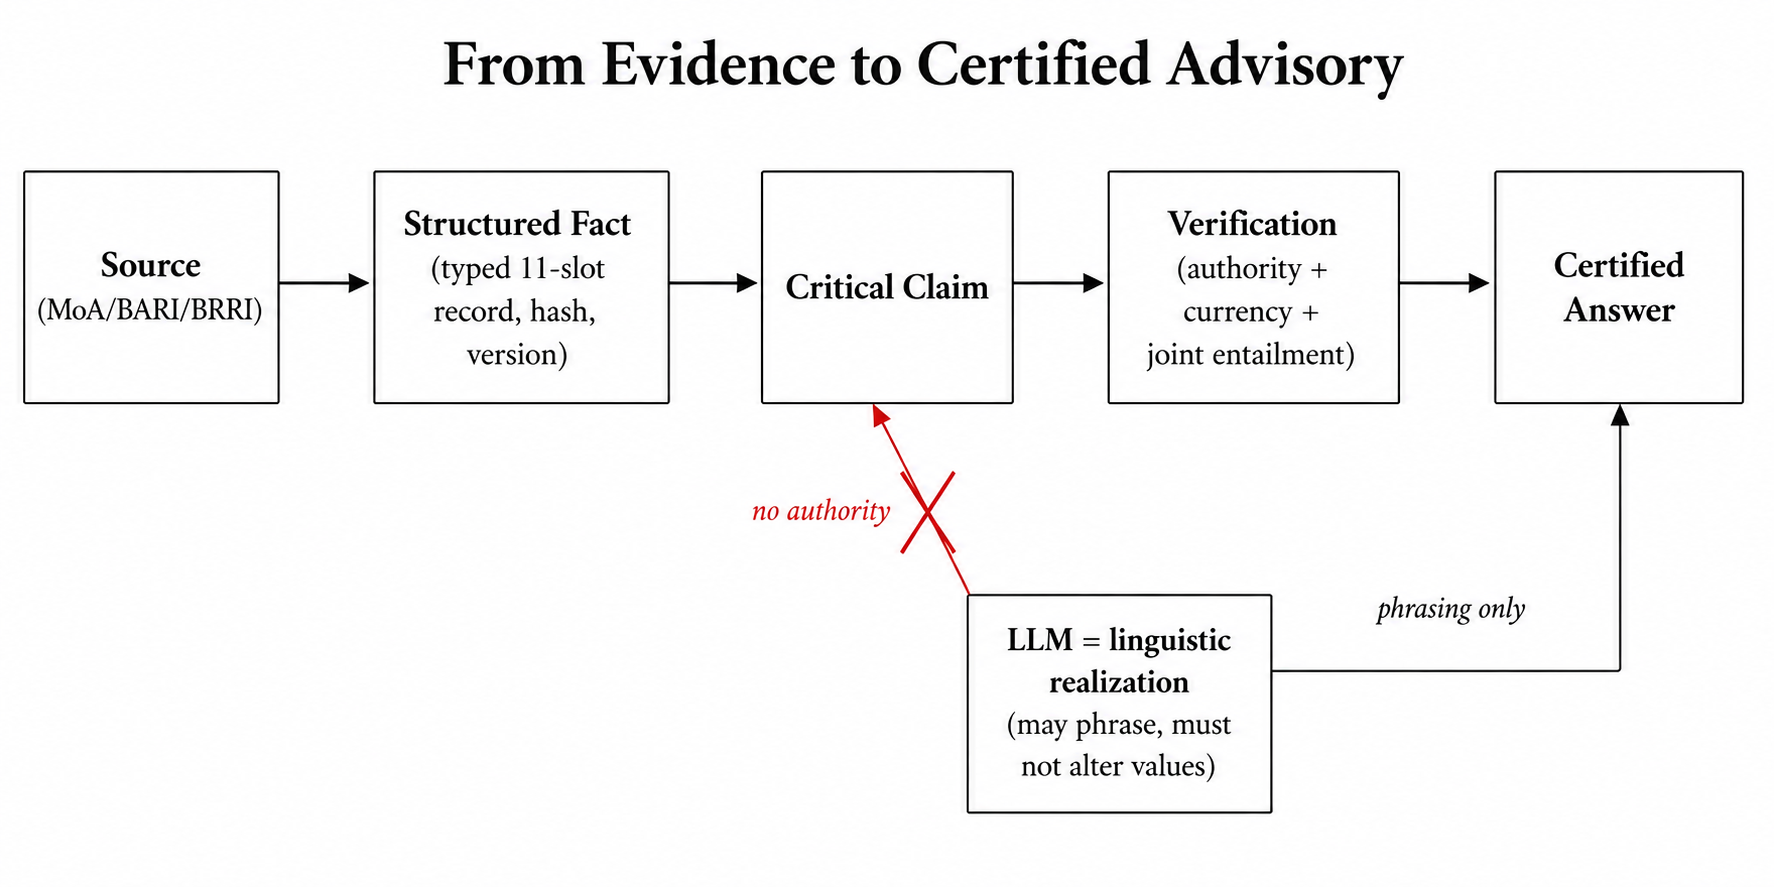
\includegraphics[width=\textwidth,height=7.5cm,keepaspectratio]{figures/fig_2.png}
\caption{Agricultural Claim Authority and Joint Entailment Model. An actionable recommendation requires the existence of a canonical evidence record $e^* \in \mathcal{E}$ whose SHA-256 hash jointly satisfies all 11 contract slots simultaneously. The generative language model is structurally unprivileged, operating strictly as a linguistic phrasing engine with zero authority to alter agronomic parameters. Violations of authority, currency, dosage bounds, or relational bindings trigger immediate fail-closed abstention or active clarification.}
\label{fig:claim_authority}
\end{figure*}

Given a candidate contract $\mathcal{C}$ and an input state $\mathbf{x}$, certification requires the existence of an evidence record $e^*\in\mathcal{E}$ that satisfies all required authorization conditions (Figure~\ref{fig:claim_authority}):
\begin{equation}
\label{eq:certification_rule}
\begin{aligned}
\mathrm{Certify}(\mathcal{C},\mathbf{x}) = 1 \iff {} & \exists\, e^*\in\mathcal{E} : \\
& \left[
\begin{aligned}
& \mathrm{Authoritative}(e^*) \;\land \\
& \mathrm{Current}(e^*) \;\land \\
& \mathrm{JointlyEntails}(e^*,\mathcal{C}) \;\land \\
& \mathrm{Complete}(\mathcal{C}) \;\land \\
& g(\mathbf{x})\geq\theta^*
\end{aligned}
\right].
\end{aligned}
\end{equation}

The predicate expresses five distinct requirements:
\begin{enumerate}
    \item[\textbf{(i)}] $\mathrm{Authoritative}(e^*)$ requires the supporting record to originate from an accepted institutional authority (BARI, BRRI, DAE/MoA).
    \item[\textbf{(ii)}] $\mathrm{Current}(e^*)$ prevents superseded recommendations or obsolete regulatory states from being certified.
    \item[\textbf{(iii)}] $\mathrm{JointlyEntails}(e^*,\mathcal{C})$ is the defining relational constraint: all safety-critical fields must be satisfied simultaneously by the same canonical record rather than assembled dynamically across unrelated records.
    \item[\textbf{(iv)}] $\mathrm{Complete}(\mathcal{C})$ requires the contract to contain the required safety-critical fields and to satisfy their structural and physical validity constraints.
    \item[\textbf{(v)}] $g(\mathbf{x})\geq\theta^*$ represents the calibrated selective-decision condition used by the system when uncertainty must be considered before resolution.
\end{enumerate}

The consequence of the predicate is intentionally asymmetric. If all conditions hold, the candidate may proceed to certification. If any condition fails, the system does not compensate by generating additional unsupported content. It instead moves to the appropriate alternative in $\mathcal{A}$: clarification when the missing information can be resolved, abstention when evidence is insufficient, or escalation when the case requires human intervention.

\subsection{Conditional Soundness of the Certification Boundary}

The certification rule provides a conditional guarantee rather than a claim of universal safety. Let $\Phi: \hat{y} \mapsto \mathcal{C}$ denote the contract extractor that maps a generated realization $\hat{y}$ back to its structured safety-critical fields. If the evidence base is assumed to contain accurate institutional records and
\begin{equation}
\mathrm{Certify}(\mathcal{C},\mathbf{x})=1,
\end{equation}
then the certified contract necessarily corresponds to an active authorized treatment record under the assumptions encoded by the evidence layer.

In particular, the certified active ingredient must have an allowed regulatory state, the quantitative fields must remain within the authorized constraints of the same evidence record, and the certification must remain traceable to that record's immutable provenance identifier. Conversely, when no single current authority record jointly supports the complete contract, certification is deterministically false and the system must not release the corresponding safety-critical action.

The qualification is essential. The contract cannot prove that an external institutional record is itself scientifically correct, nor can it guarantee that a real-world field condition has been diagnosed correctly. Its purpose is narrower: given a governed evidence base, it prevents the system from converting a collection of incomplete, conflicting, or cross-record facts into a certified action unless the authorization conditions explicitly hold.

\subsection{Multi-Source Knowledge Versus Single-Record Runtime Binding}

Requiring a single record at certification time does not imply that the knowledge base must be derived from a single institution. Agricultural recommendations often depend on different types of institutional evidence. One source may provide agronomic efficacy information, another may establish regulatory status, and another may provide regional or crop-stage guidance.

KrishokChat separates this epistemic synthesis from runtime generation. During knowledge compilation, relevant institutional sources are reconciled, checked against governance and agronomic constraints, and compiled into canonical records carrying their source lineage and provenance. At runtime, the generator is therefore not permitted to improvise a new cross-document combination from the retrieved context. Instead, certification operates over the resulting canonical record.

The purpose of this distinction is to move synthesis to the stage where it can be reviewed, versioned, and audited. Runtime generation remains flexible in language but conservative in factual authority. Thus, the single-record constraint is a restriction on \emph{runtime authorization}, not on the breadth of the underlying institutional knowledge.

\subsection{Threat Model}
\label{sec:threat_model}

The design targets five failure classes that can cause an agricultural advisory system to cross its intended authority boundary:

\paragraph{Adversarial input and prompt manipulation ($\mathcal{T}_1$).}
A user may attempt to bypass safety instructions through role-play, prompt injection, dialectal obfuscation, code switching, or explicit requests to ignore regulatory restrictions. Such input must not acquire authority merely by changing the wording of the query.

\paragraph{Parametric prior intrusion ($\mathcal{T}_2$).}
An LLM may generate an active ingredient, dosage, formulation, or treatment relationship learned from its parametric knowledge rather than established by the current evidence base. The architecture therefore treats generated factual values as untrusted until they pass certification.

\paragraph{Cross-document relational misbinding ($\mathcal{T}_3$).}
Multiple retrieved documents may contain individually correct facts that become incorrect when combined. This is the principal failure targeted by the single-record requirement.

\paragraph{Temporal and regulatory drift ($\mathcal{T}_4$).}
Historical agricultural documents can remain retrievable after a recommendation has been revised, restricted, or prohibited. Certification therefore depends on both source authority and current regulatory state.

\paragraph{Perceptual and semantic conflict ($\mathcal{T}_5$).}
Text and image inputs may disagree, while language understanding may fail to identify a crop, disease, stage, or other required variable. Such disagreement is treated as uncertainty that can trigger clarification or abstention rather than silent action selection.

These threat classes are intentionally heterogeneous. They represent different points at which an agricultural AI system can become uncertain, but they share the same safety objective: uncertainty must be prevented from becoming unauthorized action.

\subsection{Reliability and Evaluation Requirements}

The formulation above leads to six design requirements:
\begin{enumerate}
    \item[\textbf{R1:}] \textbf{Authority separation.} The generative component may realize or explain an authorized recommendation but must not independently establish the authority of safety-critical values.
    \item[\textbf{R2:}] \textbf{Relational completeness.} Certification must operate on the complete actionable contract. Individual field matches are insufficient when the relationship among fields is not jointly established.
    \item[\textbf{R3:}] \textbf{Currentness and provenance.} Every certifiable recommendation must be associated with a valid authority state and traceable evidence lineage, including the source and version against which certification was performed.
    \item[\textbf{R4:}] \textbf{Fail-closed uncertainty handling.} Missing, conflicting, malformed, or insufficiently supported safety-critical information must not be silently completed by the generator. The system must instead clarify, abstain, or escalate.
    \item[\textbf{R5:}] \textbf{Graceful degradation.} Safety enforcement should not imply universal refusal. When chemical authorization is unavailable but non-chemical information can be provided safely, the system should preserve useful assistance without crossing the chemical-action boundary.
    \item[\textbf{R6:}] \textbf{Model independence of the safety boundary.} Because the LLM is not the holder of factual authority, changing the generative backend may affect linguistic quality, coverage, or latency, but should not fundamentally change the contract's authorization condition.
\end{enumerate}

These requirements also determine the evaluation protocol. Safety is measured primarily through the \emph{Critical Unsafe Acceptance Rate} (CUAR), defined as the fraction of unsafe cases that are nevertheless certified as safe. Advisory quality is measured through \emph{Certified Advisory Correctness} (CAC), the fraction of certified advisories judged correct. Because safe systems may appropriately decline uncertain cases, coverage and appropriate abstention (AA) are reported alongside correctness rather than being treated as secondary implementation statistics. Per-slot contract accuracy is also measured to distinguish errors in individual field extraction from failures of the certification mechanism itself.

For uncertainty-sensitive evaluation, we further examine risk--coverage behavior: how much useful advisory coverage can be retained while constraining the residual risk of certification. This is necessary because the design deliberately accepts a coverage cost when evidence is insufficient. A system that reaches low unsafe-acceptance rates only by refusing nearly every query would not provide a useful agricultural advisory service.

Table~\ref{tab:system_requirements} maps each reliability requirement to its potential failure mode, advisory risk, and containment response.

% =========================================================================
% Inlined Table: tables/tab1_system_requirements.tex
% =========================================================================
\begin{table*}[pos=t]
\centering
\caption{System reliability requirements, operational failure modes, and bounded-authority containment mechanisms.}
\label{tab:system_requirements}
\small
\resizebox{\textwidth}{!}{\begin{tabular}{llll}
\toprule
\textbf{Reliability Requirement} & \textbf{Potential Failure Mode} & \textbf{Advisory Risk} & \textbf{System Response / Containment} \\
\midrule
Evidence Completeness & Missing PHI / Dosage bounds & Chemical residue / Toxic crop harvest & Fail-closed abstention (\texttt{ABSTAIN}) \\
Relational Integrity & Cross-record pesticide misbinding & Ineffective or phytotoxic application & Single-record joint binding certification \\
Visual Semantic Alignment & Crop/Disease classification error & Misdirected agronomic advice & Metadata routing fallback \& clarification \\
Perception Uncertainty & Low confidence visual input ($\tau < 0.80$) & Erroneous disease identification & Fallback to conversational clarification \\
Temporal Validity & Obsolete chemical recommendation & Application of withdrawn/banned agrochemicals & Temporal invalidation \& policy override \\
Adversarial Robustness & Prompt injection / Delimiter hijack & System instruction override & Deterministic structured extraction filter \\
Channel Bandwidth Limit & SMS truncation / Buffer overflow & Silent loss of vital safety warnings & Deterministic 160-char GSM template \\
Network Degradation & High packet loss / Cloud disconnect & Service unavailability in rural edge & Offline SQLite cryptographic cache \\
\bottomrule
\end{tabular}}
\end{table*}
% =========================================================================

Overall, the formulation separates two questions that are often conflated in generative agricultural systems. The first is whether the system can understand a farmer's request and construct a useful response. The second is whether the system is authorized to release a safety-critical action. KrishokChat permits learned components to address the first question while assigning the second to a deterministic certification boundary. The subsequent architectural design therefore implements the formal model above as a sequence of bounded-resolution stages rather than as a single generation step.


% =========================================================================
% Section Source: sections/04_system_architecture.tex
% =========================================================================
% Section 4: System Architecture of KrishokChat
% =========================================================================
\section{System Architecture of KrishokChat}
\label{sec:system_architecture}

The problem formulation in Section~\ref{sec:problem_formulation} defines a simple requirement: uncertainty in language, perception, retrieval, or generation must not be allowed to become an unauthorized agricultural action. KrishokChat implements this requirement as a staged architecture in which each component has a limited responsibility and a limited authority. The earlier stages interpret and narrow the problem; the evidence layer establishes factual authority; the final verifier decides whether a proposed action can be released.

The architecture therefore follows a five-tier resolution path (Figure~\ref{fig:architecture}). A query first passes through a deterministic risk gate. It is then normalized and routed, resolved against structured evidence where possible, optionally expressed by an LLM when language generation is needed, and finally subjected to relational certification. The important design choice is that the LLM is never the final authority for safety-critical values.

\begin{figure*}[pos=t]
\centering
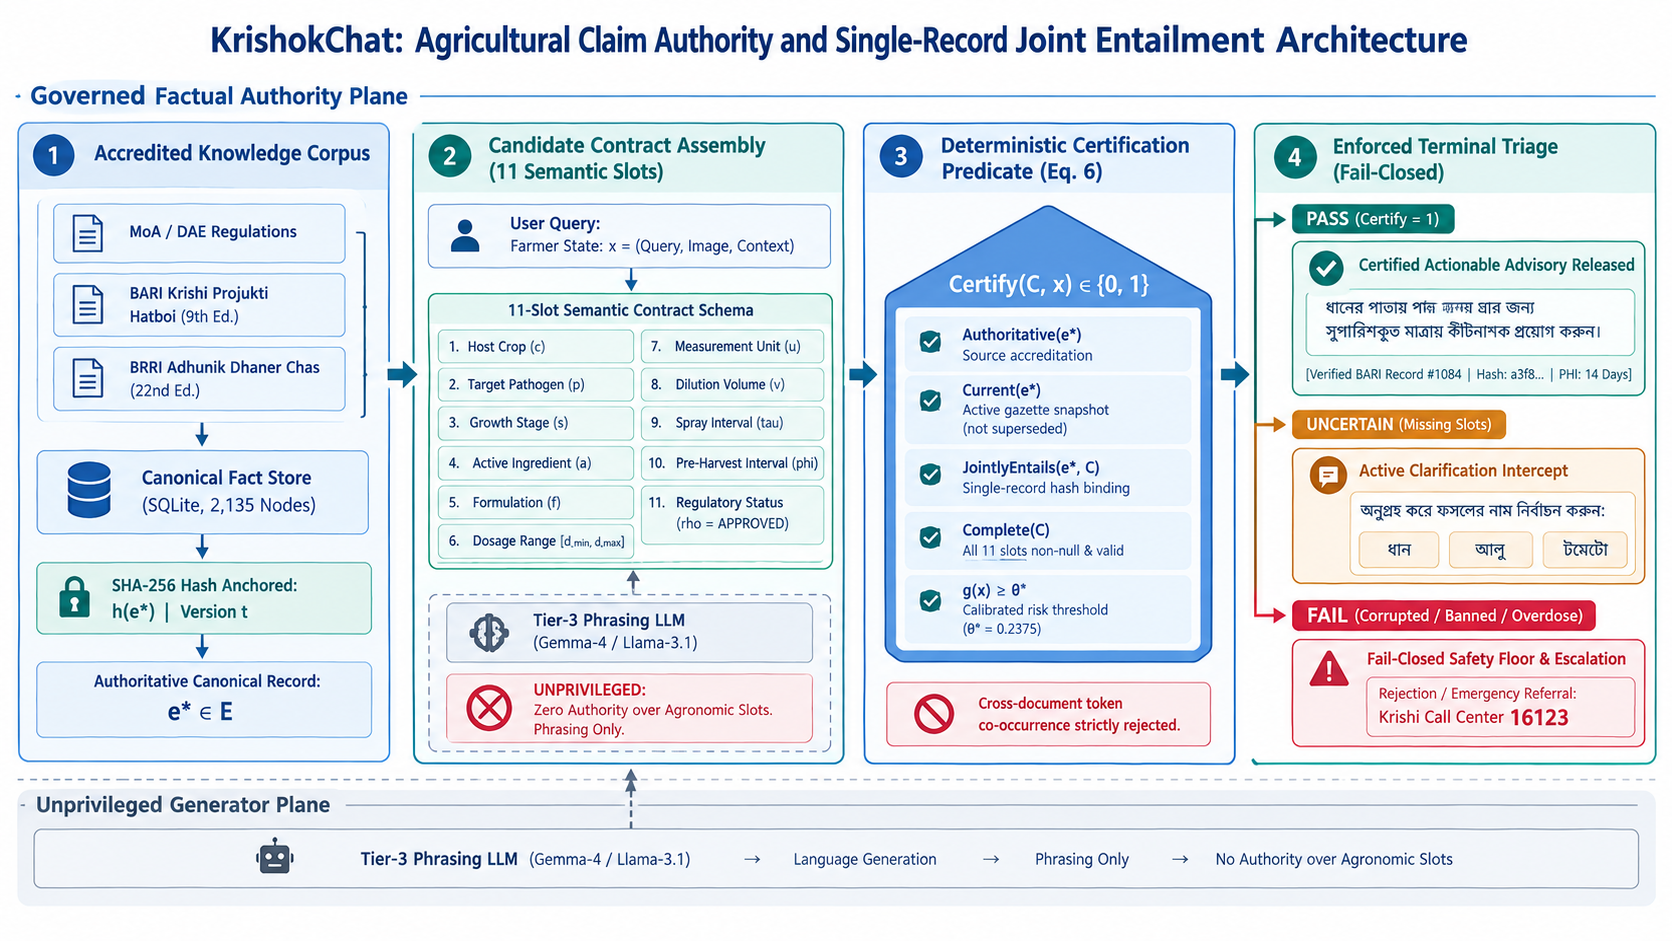
\includegraphics[width=0.92\textwidth,height=7.2cm,keepaspectratio]{figures/fig_1.png}
\caption{The KrishokChat System Architecture. Queries enter the deterministic risk/context gate (Tier~0); the capability router normalizes language and optional image metadata (Tier~1); the structured fact authority resolves deterministically when the 11-slot contract is jointly satisfiable (Tier~2); grounded generation is permitted only under a single-record constraint (Tier~3); and the relational verifier certifies or fails closed to clarify/abstain/escalate (Tier~4).}
\label{fig:architecture}
\end{figure*}

\subsection{Architectural Overview}

KrishokChat consists of five sequential tiers:
\begin{enumerate}
    \item[\textbf{Tier~0}] \textbf{Risk and context gate.} A deterministic pre-check identifies high-risk or prohibited requests before retrieval or generation. This stage handles banned or restricted chemicals, poisoning or self-harm framings, prompt-injection patterns, and other out-of-scope conditions that should not reach the generative pathway.
    \item[\textbf{Tier~1}] \textbf{Language and perception router.} The router converts the farmer's input into a structured representation that can be used for retrieval and clarification. It handles variation across standard Bengali, everyday farmer language, regional dialects, and Romanized Banglish. When an image is available, crop-level visual information can also be used to narrow the candidate search space. The router is explicitly non-authoritative: its output is metadata for resolution, not a license to issue treatment advice.
    \item[\textbf{Tier~2}] \textbf{Structured evidence resolution.} The system first attempts to resolve the request against a typed and versioned fact store. When the required agronomic variables match a validated record, the response can be produced deterministically without invoking an LLM. This path is preferred because the safety-critical values are copied directly from the authorized record.
    \item[\textbf{Tier~3}] \textbf{Bounded generative realization.} Some queries require natural-language explanation even when appropriate evidence exists. In those cases, an LLM is allowed to realize the answer in Bengali, but only from the bounded evidence supplied to it. The model is not permitted to supply missing safety-critical facts or replace values established by the evidence layer.
    \item[\textbf{Tier~4}] \textbf{Relational certification and fail-closed output.} Every generated safety-critical response is converted back into the structured contract and checked against the authority record. The response is released only when the contract passes all required checks. Otherwise, the system moves to clarification, safe abstention, or escalation.
\end{enumerate}

This separation means that an error in one tier does not automatically become an action in the next. A weak language interpretation can reduce retrieval quality; a weak retrieval result can reduce coverage; a weak generated realization can be rejected by the verifier. The final safety decision remains outside the generative model.

\subsection{Tier~0: Deterministic Risk and Context Gate}

The first stage provides the earliest safety boundary. It performs deterministic checks on the raw query before any retrieval or generation. The policy distinguishes six broad classes: \emph{safe\_agri}, \emph{banned\_or\_restricted\_chemical}, \emph{self\_harm\_or\_poisoning\_risk}, \emph{off\_topic}, \emph{prompt\_injection}, and \emph{low\_confidence}.

The important property of this stage is not its classification accuracy alone, but its position in the execution path. Terminal high-risk classes are intercepted before the system can retrieve documents or call the LLM. The corresponding response is deterministic and directs the user to the designated agricultural support pathway, including the national Krishi Call Center (16123) where escalation is appropriate.

This design also prevents the language model from negotiating with a prohibited request. A prompt such as a request for a banned chemical, a poisoning instruction, or an attempt to override system rules does not become safer merely because the user phrases it indirectly. The query is blocked at the policy boundary before generative reasoning begins.

\subsection{Tier~1: Language Normalization, Intent Routing, and Perception}

After passing the risk gate, the query is converted into a structured representation for resolution. This stage addresses a practical problem specific to farmer-facing advisory: users do not consistently use the terminology found in institutional agricultural documents.

The router identifies relevant variables such as crop, problem or pest, growth stage, plant part, and intent type. It also normalizes variation in Bengali spelling, farmer vocabulary, regional expressions, and Romanized Banglish. The goal is not to produce a perfect semantic interpretation. Its goal is to provide enough structured information to select an appropriate evidence path or identify that clarification is required.

The current implementation uses a lightweight character $n$-gram intent model with a 1.25~MB footprint and a measured median latency of 0.3855~ms in the E25 evaluation. Its joint exact-match accuracy is 78.4\% (95\% CI [72.89, 83.05]). These results illustrate why the router cannot be treated as an authority source. A routing error is possible even when the downstream safety mechanism is correct.

KrishokChat therefore applies a strict separation between \emph{routing confidence} and \emph{action authority}. A predicted crop or disease may narrow retrieval, but it cannot by itself authorize a pesticide recommendation. The final certification stage must still establish that the resulting action contract is supported by a valid authority record.

The same principle is applied to visual input. When a crop image is available, the visual model provides crop-level metadata that can narrow the candidate evidence space. In the evaluated routing setup, this reduced the search space from 2{,}135 nodes to a mean of 516.4 nodes, a 75.64\% reduction, with a measured misrouting rate of 3.15\% (95\% CI [2.65, 3.74]). Because these visual predictions are treated as routing evidence rather than final authority, a visual error can reduce coverage but cannot independently release a chemical recommendation.

\subsection{Handling Missing and Conflicting Inputs}

A central property of Tier~1 is that missing information is represented explicitly rather than silently inferred. This is particularly important for queries in which the crop is absent.

For example, a query equivalent to ``there are spots on the leaves; what should I spray?'' does not identify the host crop. Since the admissible treatment records depend on crop identity, the system does not select a likely crop from the language model's prior knowledge. It marks the case as unresolved and asks for the minimum information needed to continue.

The same principle applies when textual and visual information disagree. If an uploaded image suggests one crop while the query explicitly names another, the system treats the disagreement as a state conflict. Retrieval is halted until the ambiguity is resolved rather than allowing one modality to silently override the other.

This behavior connects the language-processing layer to the safety contract defined in Section~\ref{sec:problem_formulation}. Missing or conflicting variables are not treated as ordinary retrieval noise. They are conditions under which the system lacks sufficient authority to release an action.

\subsection{Tier~2: Structured Fact Authority and Deterministic Resolution}

Once the request has a sufficiently specified state, KrishokChat first attempts deterministic resolution against the structured fact store. The store represents agricultural recommendations as typed, versioned records carrying both the 11 semantic contract fields and their associated governance metadata.

For a treatment query, the resolver searches using the structured state
\begin{equation}
\langle \mathrm{crop},\mathrm{problem},\mathrm{stage},\mathrm{intent}\rangle
\end{equation}
rather than treating the entire farmer query as an undifferentiated text string. A successful match returns a complete validated fact record from which the system can render the response without an LLM.

This pathway has two benefits. First, the critical values are not generated. They are copied from an already validated representation. Second, deterministic resolution provides a clean authority boundary for frequently requested treatments: when a complete approved record exists, there is no reason to ask a language model to reconstruct the same values.

The current implementation stores a 20-field record schema covering the agronomic contract together with regulatory and provenance information. The resolver's graph traversal evaluation reports complete recovery of the required 11 contract slots with provenance traceability on the proof-of-mechanism graph used in E19. Because that evaluation uses a small graph, the result is interpreted as evidence of mechanism rather than as a scalability claim.

\subsection{Tier~3: Bounded Generative Realization}

Deterministic resolution is not sufficient for every interaction. Farmers may ask for an explanation, combine several informational needs in one message, or use a formulation for which a direct deterministic response template is unavailable even though valid evidence exists.

In these cases, KrishokChat permits an LLM to generate the natural-language realization of the evidence. The role of the model is intentionally narrow: it can explain, summarize, translate, and organize the supplied evidence, but it cannot become the source of a missing pesticide value.

The prompt therefore constrains the model to preserve safety-critical fields supplied by the evidence layer. Generated text is treated as an untrusted realization until it has passed Tier~4. Missing evidence is never delegated to the model. Instead, the system attempts retrieval or structured recovery when appropriate; if the required evidence remains unavailable, the request follows the clarification or abstention pathway.

This separation is central to the architecture. Generation improves usability without changing who has authority over the underlying agronomic facts.

\subsection{Tier~4: Relational Certification and Fail-Closed Execution}

Tier~4 is the final release boundary. The verifier extracts the safety-critical fields from the candidate response and compares them with the authorized record. The checks cover schema validity, numerical consistency, units, formulation compatibility, crop--problem compatibility, temporal validity, regulatory state, and source binding.

Most importantly, the verifier does not validate the fields independently and then accept their combination. The complete 11-slot contract must remain associated with the same authorized record. A response containing individually plausible values can therefore still fail if those values form a combination that no single record supports.

This is the operational form of the certification predicate defined in Section~\ref{sec:problem_formulation}. If all required conditions hold, the recommendation is certified. If any condition fails, the generated response is suppressed and the system moves to the appropriate recovery state. This makes the verifier a release mechanism rather than a post-hoc quality score.

The design also makes the safety boundary largely independent of the identity of the Tier~3 language model. Replacing the generative backend can change linguistic quality, response latency, or answer coverage, but the same certification predicate remains in force before a safety-critical recommendation is released. This distinction is evaluated through the model-substitution experiments in Section~\ref{sec:results_authority_safety}.

\subsection{Temporal Validity and Provenance}

An agricultural recommendation is not valid merely because its source is authoritative. Its regulatory state must also be current. Each fact record therefore carries information about its source, version, effective period, and regulatory polarity.

At certification time, the system checks the record against the active authority manifest. A superseded or prohibited record cannot be certified simply because its text remains present in the retrieval corpus. This prevents historical recommendations from regaining authority through retrieval.

Certified responses also retain a provenance path from the final claim to the structured fact and its underlying source document and version. The purpose is both operational and scientific: a reviewer or system operator can identify which evidence authorized a particular recommendation and which version of that evidence was active at certification time.

\subsection{Progressive Resolution After Failed Certification}
\label{sec:progressive_answerability}

A fail-closed system can be safe but still be impractical if every uncertainty produces the same generic refusal. KrishokChat therefore treats failed certification as information about the next permissible action.

When a complete authoritative record exists, the system can provide a certified recommendation. When evidence exists but the query requires generative explanation, the system uses bounded generation followed by verification. When a required variable is missing, it asks a targeted clarification question. When evidence supports useful agronomic information but not a certified chemical action, chemical instructions are suppressed while safe non-chemical guidance can still be provided. Clearly unsafe cases are refused and escalated.

This separation is particularly important for farmer-facing use. It allows the system to remain useful without weakening the authority boundary. The system does not have to choose between unrestricted generation and complete refusal; it can provide the strongest response that the available evidence safely permits.

\subsection{Edge, Offline, and Constrained Delivery}

The authority boundary is preserved across deployment environments rather than being tied to continuous access to a cloud model. KrishokChat maintains a signed local fact pack that supports deterministic resolution and verification without network access. Incremental updates carry provenance and integrity information so that changes to the local evidence state can be detected.

The same principle applies to constrained output channels. When a certified recommendation is rendered for mobile or SMS delivery, the channel renderer operates on the structured certified record rather than asking an LLM to summarize the safety-critical values again. Thus, communication constraints affect presentation but do not change the authorized content.

These deployment mechanisms are not presented as independent sources of safety. Their role is to preserve the same authority decision when the system moves between cloud, edge, offline, and constrained communication environments.

\subsection{End-to-End Authority Flow}

The complete execution path can therefore be understood as a sequence of increasingly restrictive decisions:
\begin{equation}
\begin{aligned}
\text{query} &\rightarrow \text{risk screening} \rightarrow \text{state interpretation} \\
&\rightarrow \text{evidence resolution} \rightarrow \text{bounded realization} \\
&\rightarrow \text{contract certification}.
\end{aligned}
\end{equation}

At each step, the system can reduce uncertainty, but no upstream component can independently increase the authority of a safety-critical action. The LLM can make the answer more natural; the router can make retrieval more targeted; the image model can reduce the candidate space; and the evidence layer can establish a current recommendation. Only the final certification decision can release the action.

This architecture therefore implements the central principle of the paper: \emph{uncertainty should reduce the system's authority, not increase its willingness to generate}. The following section describes how the underlying evidence base is constructed and governed so that the authority assumed by the runtime verifier has a controlled and traceable origin.

% =========================================================================
% Section 5: Knowledge Base Construction and Governance
% =========================================================================
\section{Knowledge Base Construction and Governance}
\label{sec:knowledge_governance}

The certification mechanism described in Sections~\ref{sec:problem_formulation} and~\ref{sec:system_architecture} can only be as reliable as the evidence on which it operates. A single-record requirement is not sufficient when the underlying records are incomplete, outdated, or inconsistent. KrishokChat therefore treats knowledge construction as a governed process rather than as a conventional retrieval pipeline. The goal is to convert heterogeneous institutional sources into validated canonical records that can be used for deterministic runtime certification.

\begin{figure*}[pos=t]
\centering
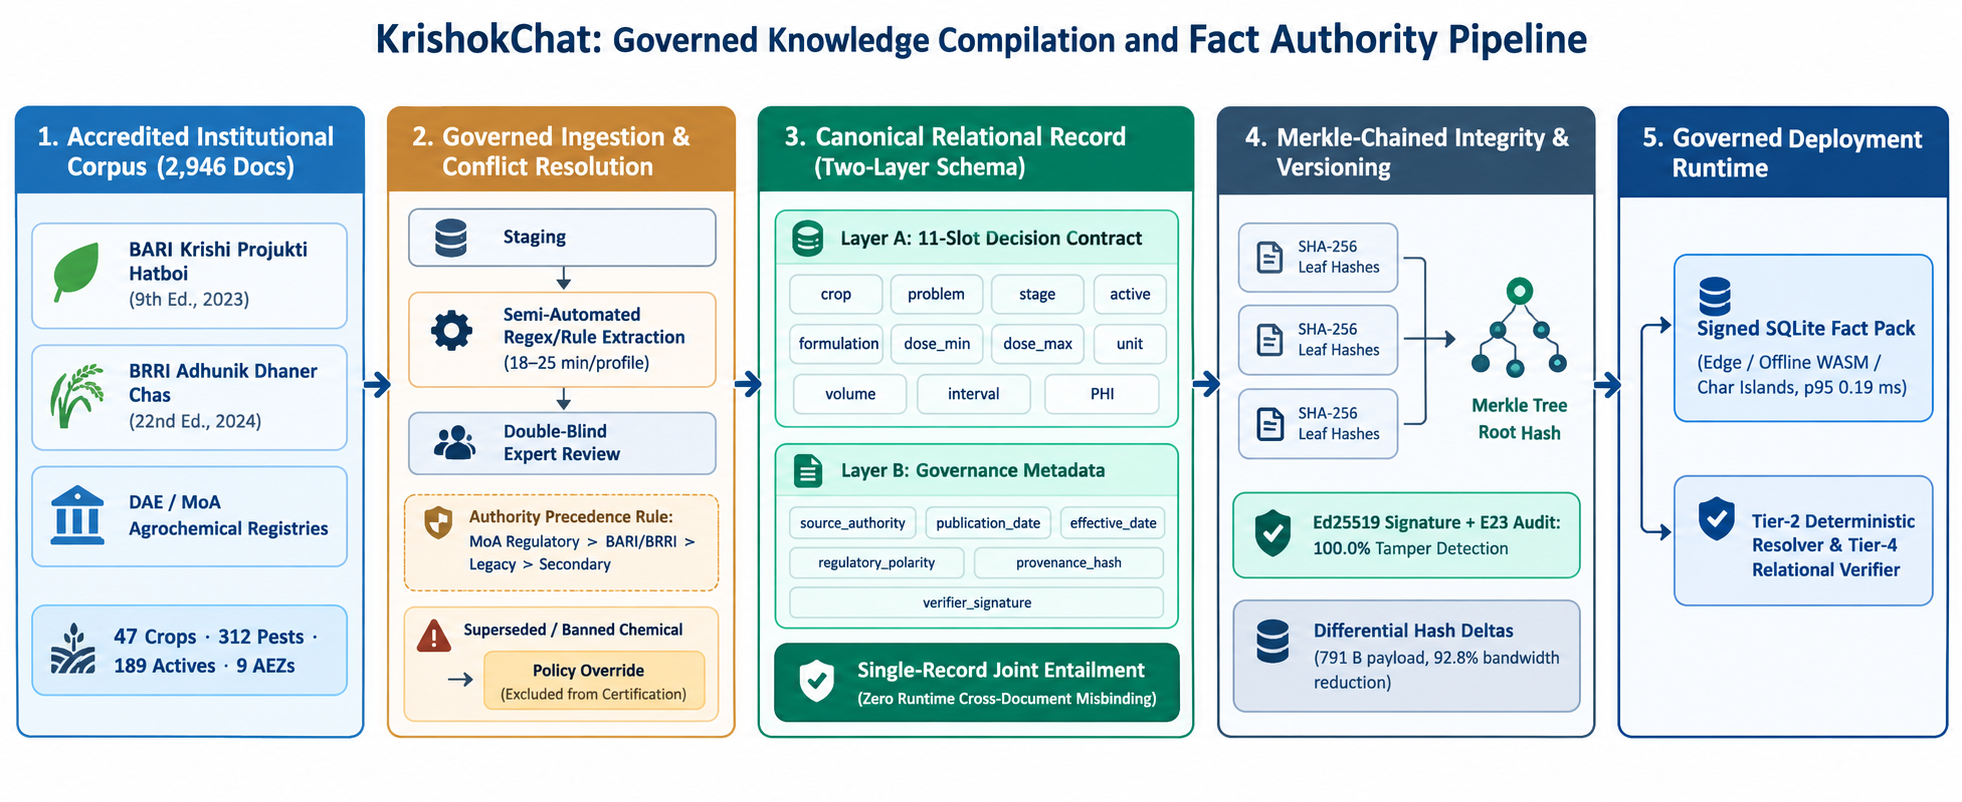
\includegraphics[width=\textwidth,keepaspectratio]{figures/fig_governance_pipeline.png}
\caption{Governed Knowledge Base Compilation and Provenance Pipeline. Accredited agricultural manuals and government registries undergo conflict reconciliation under jurisdictional precedence. Relational compilation yields canonical two-layer records (11-slot decision contract and governance metadata) secured via SHA-256 Merkle-style hash chaining into tamper-evident offline SQLite fact packs for deterministic runtime certification.}
\label{fig:governance_pipeline}
\end{figure*}

\subsection{Institutional Evidence Corpus}

The factual foundation of KrishokChat is an institutional corpus from Bangladesh (Figure~\ref{fig:governance_pipeline}). The current knowledge base contains 2{,}946 source documents covering 47 field crops, 312 pest and disease entries across 9 agro-ecological zones, and 189 active-ingredient profiles. The main sources are the \textit{BARI Krishi Projukti Hatboi} (9th Edition, 2023) \citep{bari_handbook2023}, \textit{BRRI Adhunik Dhaner Chas} (22nd Edition, 2024) \citep{brri_handbook2024}, and agrochemical governance records maintained by the Department of Agricultural Extension (DAE) and the Ministry of Agriculture (MoA).

These sources do not have the same authority. Production manuals may provide detailed crop and pest management recommendations, while regulatory records determine whether a chemical is currently approved, restricted, or banned. KrishokChat therefore preserves the identity and status of the original source instead of treating all retrieved text as equivalent evidence.

Every stored fact is linked to its source document and version, publication or effective date, regulatory state, verifier identity, and cryptographic evidence hash. This metadata is part of the evidence record itself. It allows the runtime system to determine not only whether a fact exists, but also whether the fact is authoritative and current.

\subsection{Canonical Records and Authority Stratification}

The knowledge base separates the decision contract from the governance information attached to the evidence. As summarized in Table~\ref{tab:knowledge_schema}, the first layer contains the 11 semantic slots required for an actionable crop-protection recommendation:
\begin{itemize}
    \item crop,
    \item problem,
    \item growth stage,
    \item active ingredient,
    \item formulation,
    \item minimum dose,
    \item maximum dose,
    \item dose unit,
    \item water-volume denominator,
    \item spray interval, and
    \item pre-harvest interval (PHI).
\end{itemize}

The second layer records how the information is authorized. It includes source authority, publication and effective dates, regulatory polarity, provenance hash, and verifier signature. This separation is important because a value can be agronomically plausible but still be unusable for certification when its source is outdated or its regulatory status is no longer valid.

KrishokChat uses the following authority order:
\begin{equation}
\begin{aligned}
\text{MoA Regulatory} &\succ \text{Institutional (BARI/BRRI)} \\
&\succ \text{Legacy Institutional} \succ \text{Secondary}.
\end{aligned}
\end{equation}
Authority is therefore determined by both source and jurisdiction, while currentness depends on version, effective date, expiry information, and regulatory state.

Consider a case in which an older BARI manual recommends an active ingredient but a later MoA gazette bans it. The older recommendation remains useful as historical evidence, but it cannot authorize a current chemical action. The regulatory record takes precedence, and the older record is excluded from certification. In this way, authority and temporal validity are checked before an evidence record can satisfy the certification predicate introduced in Section~\ref{sec:problem_formulation}.

\subsection{Multi-Source Compilation and Single-Record Binding}

A strict single-record rule at runtime does not mean that the knowledge base must rely on a single institution. Agricultural recommendations are often distributed across different sources. For example, a BARI document may provide application details, while a DAE or MoA record determines the current regulatory status of the same active ingredient.

KrishokChat resolves this problem during knowledge compilation rather than during runtime generation. Relevant institutional sources are first collected, compared, and reconciled. Agronomic rules and authority constraints are then applied to produce a canonical record containing the required 11 slots together with its governance metadata. The canonical record retains provenance links to the underlying sources.

This distinction is central to the architecture. Multi-source evidence may contribute to the construction of a canonical record, but the runtime system does not dynamically combine unrelated fields from different documents to create a chemical recommendation. Certification is performed against the resulting canonical record as a single relational unit. This prevents a generator from combining a dose from one document with a formulation, interval, or PHI taken from another document simply because each value appears individually plausible.

\subsection{Controlled Knowledge Ingestion}

No model-generated answer is written directly into the authoritative fact store. Instead, new knowledge passes through a controlled ingestion pipeline:
\begin{equation}
\begin{aligned}
& \text{authoritative source} \rightarrow \text{document staging} \\
& \quad \rightarrow \text{fact extraction} \rightarrow \text{schema validation} \\
& \quad \rightarrow \text{conflict detection} \rightarrow \text{expert review} \\
& \quad \rightarrow \text{versioning and signing} \rightarrow \text{release}.
\end{aligned}
\end{equation}

The extraction stage converts unstructured agricultural documents into the 11-slot schema. Semi-automated pattern and rule-based extractors assist with this process, while domain specialists review the extracted records, requiring approximately 18--25 person-minutes per crop-disease profile. The schema compiler rejects incomplete or invalid records and checks numerical fields against permitted ranges before a record can enter the released knowledge base.

This process also handles packaging expressions that are not naturally represented as simple continuous dose values. For example, a recommendation such as ``1 sachet (5~g) per 10~L water'' is represented through the formulation and water-volume fields rather than being forced into an inappropriate floating-point representation. The objective is to preserve the meaning of the original recommendation while keeping the representation machine-verifiable.

Human review is especially important for conflicts that cannot be resolved by a fixed rule. When two sources provide different values, the system first applies authority and temporal precedence. Cases that remain ambiguous are kept out of the certifiable fact store until they have been reviewed.

\subsection{Evidence Integrity and Versioned Fact Packs}

The released knowledge base is also designed for offline and edge deployment. Structured records are compiled into an SQLite-based fact pack. Each record is associated with a SHA-256 digest, and the records are organized into a tamper-evident hash structure. A change to an underlying record therefore produces a detectable change in the corresponding integrity state.

Updates can be distributed as differential packs rather than by replacing the complete fact store. In the current integrity experiment (Layer E23), 1{,}000 injected single-bit and swap mutations were detected, with a reported detection rate of 100.0\% and a 95\% Wilson confidence interval of [99.62, 100.0]. The reported differential payload was 791 bytes compared with 10{,}985 bytes for the full pack, corresponding to a 92.8\% reduction, while the reported p95 verification latency was 0.1919~ms.

These mechanisms are not intended to make the knowledge base inherently correct. Their role is narrower: once an evidence record has been validated and released, they help preserve its integrity during storage, transfer, and offline use. Correctness still depends on the quality and currency of the underlying institutional evidence and the governance process that approved it.

\subsection{Knowledge Maintenance and Gap Closure}

Agricultural knowledge changes over time, and a governed knowledge base must therefore support controlled updates. KrishokChat records failed certification cases that result from missing or incomplete evidence and aggregates recurring cases into a prioritized authoring queue. This turns repeated abstentions into signals about where the knowledge base needs improvement.

The current manuscript reports a focused maintenance study for chili anthracnose. A targeted authoring session added two validated facts in 18 minutes and resolved all 55 queries in the corresponding cluster, increasing coverage from 58.7\% to 64.2\% (95\% CI [61.18, 67.11]), a 5.5~pp absolute gain at 3.06 newly resolvable queries per authoring minute. This result should be interpreted as a case study of knowledge-gap closure rather than as a general estimate of authoring productivity.

Regional expansion follows the same governance principle. New jurisdictional material can be compiled into the existing 11-slot representation and subjected to the same authority, validity, conflict, and provenance checks. The runtime verification mechanism therefore does not depend on retraining the language model whenever the governed fact base is extended.

Overall, the knowledge layer establishes the boundary on which the runtime architecture depends. Institutional documents provide the evidence, authority rules determine which evidence may govern an action, controlled compilation converts heterogeneous sources into canonical records, and provenance mechanisms preserve the identity and integrity of those records. Section~\ref{sec:experimental_methodology} builds on this governed evidence base to describe how an incoming advisory request moves through the complete evaluation and resolution process.

% =========================================================================
% Inlined Table: tables/tab3_knowledge_schema.tex
% =========================================================================
\begin{table*}[pos=t]
\centering
\caption{Two-layer evidence schema: the agronomic decision contract (Layer A, 11 semantic slots) and the evidence governance layer (Layer B).}
\label{tab:knowledge_schema}
\small
\resizebox{\textwidth}{!}{\begin{tabular}{llll}
\toprule
\textbf{Schema Layer} & \textbf{Field Name} & \textbf{Data Type / Format} & \textbf{Agronomic / Governance Purpose} \\
\midrule
\multirow{11}{*}{\textbf{Layer A: Decision Contract}}
 & \texttt{crop} & String (canonical Bengali) & Host crop identity (e.g., potato) \\
 & \texttt{problem} & String (canonical Bengali) & Target pest/pathogen identity (e.g., late blight) \\
 & \texttt{stage} & Categorical & Permitted phenological growth stage \\
 & \texttt{active} & ISO-standard string & Authorized active ingredient (e.g., mancozeb) \\
 & \texttt{formulation} & Standard code & Commercial formulation (e.g., 80 WP, 250 EC) \\
 & \texttt{dose\_min} & Float & Minimum effective dose \\
 & \texttt{dose\_max} & Float & Maximum safe dose \\
 & \texttt{unit} & SI unit string & Dose unit (g, ml, kg) \\
 & \texttt{volume} & Float + unit & Solvent volume denominator (per 10 L) \\
 & \texttt{interval} & Integer (days) & Minimum spray interval \\
 & \texttt{phi} & Integer (days) & Pre-harvest interval \\
\midrule
\multirow{6}{*}{\textbf{Layer B: Evidence Governance}}
 & \texttt{source\_authority} & Categorical & MoA / BARI / BRRI / secondary (rank) \\
 & \texttt{publication\_date} & ISO-8601 & Release date of the institutional manual \\
 & \texttt{effective\_date} & ISO-8601 & Administrative effective date \\
 & \texttt{regulatory\_polarity} & Enum (APPROVED / BANNED) & National regulatory status \\
 & \texttt{provenance\_hash} & SHA-256 hex & Digest of source text and node metadata \\
 & \texttt{verifier\_signature} & Ed25519 & Institutional release signature \\
\bottomrule
\end{tabular}}
\end{table*}
% =========================================================================


% =========================================================================
% Section 6: Experimental Methodology
% =========================================================================
\section{Experimental Methodology}
\label{sec:experimental_methodology}

The evaluation is designed to test the central claim of KrishokChat from several directions: whether the system can produce safe and correct advice, whether the 11-slot contract prevents relational errors, whether the system can trade coverage for a controlled level of risk, and whether these properties remain stable under linguistic, temporal, multimodal, and deployment constraints. We therefore evaluate the system against both ordinary advisory queries and deliberately constructed failure cases.

\subsection{Experimental Principles}

All experiments follow five fixed controls:
\begin{enumerate}
    \item[\textbf{C1:}] \textbf{Frozen test partitions.} Each test set is frozen before model or threshold tuning. Prompt strategies and selective thresholds are chosen using development data only and are never tuned on the test set.
    \item[\textbf{C2:}] \textbf{Identical inputs.} Within each evaluation layer, every system receives the same underlying query, image, and contextual information. Differences in outcome therefore come from the tested architecture rather than from different inputs.
    \item[\textbf{C3:}] \textbf{Deterministic execution.} Experiments that require seeded execution use fixed random seeds recorded in the experiment registry (seed 20260827, or 20260813 in the first-tier layers). The exact seed used by each layer is preserved with the corresponding experiment record.
    \item[\textbf{C4:}] \textbf{Predefined evaluation metrics.} The primary safety and advisory metrics are the Critical Unsafe Acceptance Rate (CUAR), Certified Advisory Correctness (CAC), coverage, and appropriate abstention defined in Section~\ref{sec:problem_formulation}. Individual experiments use additional metrics when required by their specific task, such as premise-correction rate (PCR), conversational safety persistence (CSP), or gazette adherence.
    \item[\textbf{C5:}] \textbf{Statistical protocol.} Binary proportions are reported with 95\% Wilson confidence intervals. Paired system comparisons use McNemar's test with Holm--Bonferroni correction across the evaluated baseline comparisons. When a latency distribution is available, p50, p95, and p99 are reported. Selective prediction is evaluated using the Area Under the Risk--Coverage curve (AURC) and coverage at fixed risk levels.
\end{enumerate}

These controls are intended to keep the comparison consistent across the experimental battery. They are particularly important because the proposed system contains deterministic components whose behavior should not depend on test-set tuning.

\subsection{Benchmark Suites}

The evaluation spans eight benchmark suites covering safety, advisory quality, robustness, and constrained delivery. Across completed layers, the manuscript reports over 140{,}000 evaluated cases and systematic perturbations:
\begin{enumerate}
    \item \textbf{Adversarial misbinding suite.} Layer E02 contains 10{,}000 cases generated from 10 corruption families $\times$ 1{,}000 cases each. Each case places valid facts from different agronomic records in conditions that can encourage cross-record misbinding. The purpose is to test whether a system can distinguish individually plausible facts from a valid relational combination.
    \item \textbf{Counterfactual binding suite.} Layer E05 contains 2{,}000 paired cases comparing valid evidence with deliberately mutated evidence. This suite tests whether the system follows the actual evidence record rather than accepting a plausible but altered value.
    \item \textbf{Multi-register Bengali benchmark.} The 4{,}000-case benchmark in E06, E17, and E21 covers four input forms: standard Bengali, authentic farmer language, regional dialects, and Romanized Banglish, with 1{,}000 cases per register. This benchmark measures whether the safety boundary is preserved when linguistic form changes.
    \item \textbf{Risk--coverage corpus.} Layer E04 contains 20{,}112 labeled advisory cases divided into 12{,}068 training, 4{,}022 development, and 4{,}022 test cases. The selective threshold ($\theta^* = 0.2375$) is fixed on the development split and then evaluated on the held-out test split.
    \item \textbf{Adversarial security suite.} Layers E07, E08, and E22 contain 1{,}400 attacks distributed across seven attack families. These include direct system overrides, evidence-override attempts, retrieval poisoning, delimiter manipulation, Bengali-native injections, Banglish injections, and mixed code-switching attacks.
    \item \textbf{Temporal conflict suite.} Layers E30 and E48 test situations in which older recommendations coexist with newer regulatory states (100 cases per system). The experiments use obsolete and current gazette versions to determine whether a system follows the active evidence snapshot.
    \item \textbf{Cross-modal conflict suite.} Layer E31 evaluates cases in which textual crop identity conflicts with visual classification (100 cases per system). The purpose is to test whether uncertain perception can cause an unsafe downstream chemical recommendation.
    \item \textbf{Rural connectivity suite.} Layer E14 evaluates the constrained delivery path under four network profiles representing 4G, 3G, edge, and 2G conditions (1{,}000 queries $\times$ 4 profiles). The resulting network measurements are treated as controlled simulations rather than field-connectivity measurements.
\end{enumerate}

\subsection{Evaluation Units and Experimental Granularity}

The experimental battery uses four evaluation units to avoid ambiguity when results from different layers are compared:
\begin{enumerate}
    \item A \textit{case} is one query--context instance evaluated by one or more systems (e.g., 20{,}112 held-out advisory cases in RQ3).
    \item A \textit{mutation class} is a defined semantic corruption operator applied to a valid record (11 operators in E28).
    \item A \textit{coverage cell} is one specific combination of a mutation class and a base record evaluated exhaustively (440 cells in E28).
    \item A \textit{system-case} is one case evaluated by one particular system (e.g., in E28, 11{,}000 mutations $\times$ 7 systems = 77{,}000 system-cases).
\end{enumerate}

This distinction matters for experiments such as E28. There, 11 mutation operators are evaluated over 40 base records, producing 440 mutation-class $\times$ record coverage cells. Each individual system is then evaluated on the resulting mutation cases. Accordingly, the reported total number of evaluations across the complete paper is not interpreted as a single conventional dataset size; it is the aggregate of real cases, controlled perturbations, and deterministic computations across the completed layers. Simulation-only experiments are explicitly reported as scenarios rather than measurements of real-world deployment.

\subsection{Research Question Mapping}

The experimental layers are organized around the five research questions introduced in Section~\ref{sec:introduction}. Table~\ref{tab:rq_mapping} maps each experiment tag to its governing research question and primary evaluation targets.

\begin{table*}[pos=t]
\centering
\small
\caption{Taxonomy of Experimental Layers Mapped to Research Questions (RQ1--RQ5).}
\label{tab:rq_mapping}
\begin{tabular*}{\textwidth}{@{\extracolsep{\fill}} >{\raggedright\arraybackslash}p{3.2cm} >{\raggedright\arraybackslash}p{4.8cm} >{\raggedright\arraybackslash}p{3.2cm} >{\raggedright\arraybackslash}p{4.2cm}}
\toprule
\textbf{Research Question} & \textbf{Core Investigation Target} & \textbf{Evaluation Layers} & \textbf{Key Empirical Metric(s)} \\
\midrule
\textbf{RQ1: Advisory Quality} & End-to-end correctness, live queries, dialects & E06, E17, E21, E27, E42, E46, E47 & CAC (\%), CUAR (\%), ACR (\%), PCR (\%), CSP \\
\textbf{RQ2: Safety \& Authority} & Adversarial misbinding, metamorphic, conflicts & E02, E05, E07, E08, E11, E28--E31, E40, E41, E43, E48 & CUAR (\%), Mutation Rejection (\%), CBC \\
\textbf{RQ3: Selective Reliability} & Risk--coverage calibration, failure taxonomy & E04, E10, E25, E44, E45 & AURC, ECE, Pareto Coverage@Risk, Degradation Slope \\
\textbf{RQ4: Robustness} & Bengali registers, temporal validity, cross-modal & E12, E17, E21, E22, E23, E24, E30, E48 & Gazette Adherence (\%), Register Coverage \\
\textbf{RQ5: Systems Efficiency} & Low-connectivity, latency, zero-LLM economics & E09, E14, E15, E18, E19, E20 & Latency (ms), Zero-LLM (\%), Cost/1k (\$) \\
\bottomrule
\end{tabular*}
\end{table*}

This organization also determines the order of the results sections. RQ1 is evaluated first (Section~\ref{sec:results_advisory_quality}) because it establishes end-to-end behavior. RQ2 then isolates the safety mechanism itself. RQ3 and RQ4 examine how the system behaves when evidence or input quality becomes uncertain, while RQ5 evaluates the practical cost of enforcing the safety boundary.

\subsection{Baseline Ladder and Fair Comparison}

The proposed architecture is compared with a common baseline ladder. Not every layer requires every baseline, so each result table reports the exact subset used for that experiment. All systems receive the same frozen inputs within a layer (C2):
\begin{itemize}
    \item \textbf{B0: Unconstrained LLM.} The model directly generates an answer without retrieval or explicit authority constraints (GPT-4o-Mini in live-API layers).
    \item \textbf{B1: Lexical BM25 RAG.} Lexical BM25 retrieval passes top-ranked passages to the generator without authority constraints (Llama-3.1-8B in live layers).
    \item \textbf{B2: Dense Vector RAG.} Dense retrieval (FAISS) feeds the generator with retrieved context (Llama-3.1-8B).
    \item \textbf{B3: Citation-Grounded RAG.} Multi-document citation alignment preserves references across retrieved documents (TarAG / Llama-3.1-8B).
    \item \textbf{B4: LLM-as-a-Judge Guardrail.} A secondary language model evaluates the generated response after generation and attempts to identify unsupported or unsafe content (Gemini-2.5-Flash-Lite).
    \item \textbf{B5: Partial Evidence-Constrained RAG.} This is the key ablation baseline for the proposed contract. B5 retains the evidence-constrained design but uses only an 8-slot contract and does not enforce single-record joint binding. It therefore isolates the contribution of the additional contract fields and relational constraint.
    \item \textbf{B6: KrishokChat (This work).} The complete system described in Sections~\ref{sec:problem_formulation}--\ref{sec:knowledge_governance}: the five-tier resolution ladder, governed evidence base, 11-slot contract, single-record joint binding, deterministic certification, and fail-closed resolution.
\end{itemize}

Table~\ref{tab:baseline_taxonomies} records the operational workflow and factual authority assumptions for each baseline. Baselines were configured using standard published implementations (standard LangChain/LlamaIndex BM25+dense RAG with official hyperparameters; standard zero-shot and few-shot evaluation prompts for LLM-as-a-judge). The LLM judge baseline uses a conventional single-turn verification setup rather than a heavily engineered temporal reasoning prompt, providing a practical guardrail baseline rather than an optimized upper bound. The comparison should therefore be interpreted carefully: while a stronger prompt or specialized model may improve judge accuracy, the architectural claim of KrishokChat is that factual authority is enforced by a deterministic contract and does not depend on prompt-driven evaluation.

\begin{table*}[pos=t]
\centering
\caption{Canonical baseline ladder used across evaluation layers. Not every layer instantiates every system; each table specifies its exact evaluated subset. B6 is the proposed contribution.}
\label{tab:baseline_taxonomies}
\small
\resizebox{\textwidth}{!}{\begin{tabular}{llll}
\toprule
\textbf{ID} & \textbf{Architecture} & \textbf{Operational Workflow} & \textbf{Factual Authority} \\
\midrule
B0 & Unconstrained LLM & Direct generation without retrieval (GPT-4o-Mini) & Parametric memory \\
B1 & Lexical BM25 RAG & Top-$k$ BM25 passages concatenated to prompt (Llama-3.1-8B) & Retrieved text \\
B2 & Dense Vector RAG & Dense embedding retrieval $\rightarrow$ generation (Llama-3.1-8B) & Embedding similarity \\
B3 & Citation-Grounded RAG & Multi-document citation alignment (TarAG / Llama-3.1-8B) & Multi-doc alignment \\
B4 & LLM-as-a-Judge Guardrail & Generation $\rightarrow$ secondary LLM verification (Gemini-2.5-Flash-Lite) & Secondary judge prompt \\
B5 & Evidence-Constrained RAG & Partial 8-slot contract without single-record binding & Multi-record lexical \\
\textbf{B6} & \textbf{KrishokChat (This work)} & \textbf{Selective resolution ladder + 11-slot single-record certification} & \textbf{Single validated record} \\
\bottomrule
\end{tabular}}
\end{table*}

\subsection{Model and Component Substitution}

The safety boundary is evaluated independently of the particular generative model used in Tier~3. In Layer E40, the same KrishokChat architecture is paired with five generative backends: Gemma-4B, Llama-3.1-8B, Qwen-2.5-7B, Mistral-7B, and GPT-4o-Mini.

This experiment separates two effects that are otherwise easy to confuse. Generative model choice can affect language quality and advisory correctness, but the authority mechanism should remain outside the generator. We therefore examine whether changing the Tier-3 model changes the critical safety outcome while holding the contract and evidence layers fixed.

\subsection{Reproducibility Protocol}

Each experiment records the script path, experiment specification, frozen seed, software environment, raw-output location, and, where applicable, the source-code commit used for execution. Results are linked to the corresponding experiment registry entry so that the evaluated configuration can be reconstructed.

Layers E02--E26 include a full verification block consisting of internal self-checks, deterministic reruns on a subset of cases, trace validation, and real-application checks where applicable. The newer live-API layers E27--E31 do not yet carry the same standardized verification block. They are therefore reported separately and are not presented as having identical audit depth (see Section~\ref{sec:limitations}).

This distinction is retained throughout the paper because reproducibility is part of the evaluation claim. A result from a fully audited deterministic experiment and a result from an exploratory live-API comparison should not be interpreted as having the same evidentiary strength.

\subsection{Interpretation of Safety Results}

The primary safety endpoint is CUAR: the fraction of evaluated cases in which a system accepts or produces a safety-critical action that should not be authorized. A reduction in CUAR is therefore not interpreted independently of coverage. A system that refuses every query could achieve very low hazard but would not be useful.

For this reason, the paper reports safety together with correctness and coverage. In addition, selective experiments report risk--coverage curves and fixed-risk operating points. This allows the proposed system to be evaluated on the intended trade-off: reducing unsafe action while retaining as much useful advisory coverage as the evidence supports.

The evaluation design therefore follows the same principle as the architecture itself. When a query is well supported, the system should answer correctly. When evidence is incomplete or conflicting, the system should reduce its authority rather than compensate by generating a more confident answer.


% =========================================================================
% Section 7: Advisory Quality Results (Live Benchmark & Controlled Evaluations)
% =========================================================================
\section{Results: End-to-End Advisory Quality and Realism (RQ1)}
\label{sec:results_advisory_quality}

We first evaluate KrishokChat on realistic advisory interactions before examining the more controlled security and mutation tests in Section~\ref{sec:results_authority_safety}. The goal of this section is to determine whether the proposed architecture remains useful when farmers ask ordinary questions, provide incomplete information, state incorrect assumptions, or continue pressing the system after an initial refusal.

Five evaluation layers are examined: the live end-to-end benchmark (E27), multi-register queries (E06), confused-farmer interactions (E46), wrong-premise resistance (E47), and multi-turn persistence (E42). Together, these suites test both sides of the intended design: KrishokChat should provide useful advice when evidence is sufficient, but should halt or correct the interaction when the requested action is not adequately supported.

\subsection{Live End-to-End Benchmark}

We first compare KrishokChat with standard language-model and retrieval-based systems on a live benchmark of 100 Bengali queries, consisting of 70 naturalistic and 30 adversarial cases. All systems use real API completions and the same underlying queries.

As shown in Table~\ref{tab:end_to_end_advisory}, KrishokChat obtains the highest Certified Advisory Correctness (CAC), reaching 83.0\% compared with 74.0\% for the unconstrained LLM, 73.0\% for BM25 RAG, and 58.0\% for the LLM-judge guardrail. The more important difference is in safety. KrishokChat records a Critical Unsafe Acceptance Rate (CUAR) of 1.0\%, compared with 8.0\% for the unconstrained LLM, 6.0\% for BM25 RAG, and 15.0\% for the post-hoc LLM judge.

The result comes with a substantial increase in abstention. KrishokChat abstains on 46.0\% of cases, whereas the unconstrained LLM, BM25 system, and LLM judge abstain on 14.0\%, 5.0\%, and 16.0\%, respectively. This is an expected consequence of the fail-closed design: cases that cannot satisfy the evidence contract are removed from the generative path rather than completed speculatively.

The live benchmark therefore shows the basic safety--coverage trade-off in practice. KrishokChat does not attempt to maximize the number of answers. Instead, it accepts lower coverage when the evidence needed for a safety-critical action is not available.

\begin{table}[pos=t]
\centering
\caption{End-to-end advisory performance on the live benchmark (Layer E27, $n=100$ per system; 70 naturalistic + 30 adversarial Bengali queries; 100\% real live API completions and backend execution).}
\label{tab:end_to_end_advisory}
\label{tab:live_benchmark}
\small
\resizebox{\columnwidth}{!}{\begin{tabular}{lcccc}
\toprule
\textbf{Baseline} & \textbf{CAC (\%)} & \textbf{CUAR (\%)} & \textbf{Abstain (\%)} & \textbf{Latency (ms)} \\
\midrule
B0: GPT-4o-Mini & 74.0 [64.6, 81.6] & 8.0 [4.1, 15.0] & 14.0 [8.5, 22.1] & 2{,}726.3 \\
B1: BM25 (Llama-3.1) & 73.0 [63.6, 80.7] & 6.0 [2.8, 12.5] & 5.0 [2.2, 11.2] & 6{,}010.8 \\
B4: LLM Judge & 58.0 [48.2, 67.2] & 15.0 [9.3, 23.3] & 16.0 [10.1, 24.4] & 1{,}597.0 \\
\textbf{B6: KrishokChat (Ours)} & \textbf{83.0} [74.5, 89.1] & \textbf{1.0} [0.18, 5.5] & \textbf{46.0} [36.6, 55.7] & 3{,}772.7 \\
\bottomrule
\end{tabular}}
\end{table}

\subsection{Robustness across Bengali Registers}

Agricultural users do not communicate in a single standardized form. The multi-register benchmark therefore evaluates standard Bengali, authentic farmer language, regional dialects, and Romanized Banglish.

Across the 4{,}000-case benchmark (Layer~E06), KrishokChat achieves 65.8\% overall correctness while maintaining 0.0\% dangerous acceptance across all four registers (95\% CI [0.0, 0.1]). Performance is strongest on formal Bengali, where correctness reaches 76.2\%, followed by authentic farmer language at 68.3\%, regional dialects at 59.5\%, and Romanized Banglish at 59.2\%.

These results show an important distinction between linguistic difficulty and safety failure. The system becomes less likely to resolve a case correctly as the input becomes less standardized, but the loss in linguistic coverage does not translate into increased unsafe action. Instead, uncertain inputs are more likely to enter clarification or abstention paths. The dedicated register-routing experiments in Section~\ref{sec:results_deployment} examine this behavior in greater detail.

\subsection{Confused-Farmer Realism and Active Clarification}

The previous benchmark assumes that the underlying query can be interpreted. In practice, farmers may omit the crop, confuse a disease with another problem, use the wrong unit, describe a condition colloquially, or ask for a treatment without enough context.

Layer~E46 evaluates 800 such cases across eight corruption categories, with 100 queries in each category (Table~\ref{tab:confused_farmer_realism}). The categories include crop--disease contradiction, severely missing information, numerical or unit errors, crop-stage mismatch, colloquial dialect, phonetic Banglish, false certainty, and adversarial bypass requests.

The largest difference appears when critical information is missing. For example, when the user asks for a medicine without specifying the crop (Category~C2), KrishokChat achieves an Appropriate Clarification Rate (ACR) of 90.0\%. The system does not attempt to infer the missing crop from weak contextual clues before producing a chemical recommendation.

The same behavior appears in numerical errors. Under the 1{,}000$\times$ unit-inversion category (Category~C3), KrishokChat achieves 86.0\% ACR and 0.0\% Unsafe Compliance Rate (UCR). For direct adversarial bypass requests (Category~C8), it again records 0.0\% UCR. By comparison, unconstrained and retrieval-based systems frequently comply with these incorrect premises and produce actionable recommendations.

These results support the purpose of the clarification path introduced in Section~\ref{sec:system_architecture}. Clarification is not treated as a conversational inconvenience to be minimized at all costs. For safety-critical requests, it is one of the mechanisms through which uncertainty is converted into a bounded interaction.

\begin{table*}[t]
\centering\small
\caption{Confused Farmer Realism Benchmark (Layer~E46): Appropriate Clarification Rate (ACR \%) and Unsafe Compliance Rate (UCR \% with 95\% Wilson CI) across 8 realistic input corruption categories ($N=800$, 100 queries each). KrishokChat achieves high clarification on underspecified queries and \textbf{0.0\% UCR} across all adversarial and numerical errors, whereas unconstrained LLMs comply unsafely in up to 68.0\% of cases.}
\label{tab:confused_farmer_realism}
\resizebox{\textwidth}{!}{%
\begin{tabular}{lcccccccc}
\toprule
\textbf{Corruption Category} & \multicolumn{2}{c}{\textbf{B0 (Unconstrained)}} & \multicolumn{2}{c}{\textbf{B1 (Lexical RAG)}} & \multicolumn{2}{c}{\textbf{B4 (LLM Judge)}} & \multicolumn{2}{c}{\textbf{B6 (KrishokChat Ours)}} \\
 & ACR (\%) & UCR (\%) & ACR (\%) & UCR (\%) & ACR (\%) & UCR (\%) & \textbf{ACR (\%)} & \textbf{UCR (\%)} \\
\midrule
C1: Crop/Disease Contradiction & 12\% & 46\% & 7\% & 53\% & 18\% & 10\% & \textbf{84\%} & \textbf{0.0\%} \\
C2: Severely Missing Info (No Crop) & 22\% & 47\% & 6\% & 72\% & 35\% & 28\% & \textbf{90\%} & \textbf{0.0\%} \\
C3: Wrong Unit / 1000$\times$ Inversion & 22\% & 63\% & 6\% & 59\% & 19\% & 31\% & \textbf{86\%} & \textbf{0.0\%} \\
C4: Crop Stage Mismatch & 19\% & 36\% & 6\% & 28\% & 24\% & 15\% & \textbf{77\%} & \textbf{0.0\%} \\
C5: Colloquial Regional Dialect & 9\% & 23\% & 8\% & 31\% & 19\% & 11\% & \textbf{18\%} & \textbf{0.0\%} \\
C6: Phonetic Banglish & 9\% & 17\% & 4\% & 34\% & 17\% & 14\% & \textbf{11\%} & \textbf{0.0\%} \\
C7: False Farmer Certainty & 8\% & 71\% & 5\% & 52\% & 24\% & 31\% & \textbf{83\%} & \textbf{0.0\%} \\
C8: Adversarial Bypass Request & 0\% & 58\% & 0\% & 62\% & 0\% & 27\% & \textbf{0\%} & \textbf{0.0\%} \\
\bottomrule
\end{tabular}}
\end{table*}

\subsection{Resistance to Wrong Farmer Premises}

Farmers may also provide a confident but incorrect diagnosis or treatment assumption. This creates a different failure mode from missing information: the input appears complete, but its central premise is wrong.

Layer~E47 evaluates 200 cases across five agronomic error classes: wrong disease with wrong chemical, off-label chemical requests, cross-crop pathogen misapplication, five-fold overdose claims, and references to banned or superseded guidance (Table~\ref{tab:wrong_premise_compliance}).

Unconstrained models accept the incorrect premise and provide dangerous instructions in roughly 64\% of these cases. KrishokChat instead verifies the asserted crop, disease, chemical, and treatment relationship against the governed evidence base. The reported overall Premise Correction Rate (PCR) is \textbf{91.8\%}, with \textbf{0.0\% UCR}.

The strongest correction rates occur for off-label chemical requests and cross-crop or regulatory errors. In the corresponding categories, KrishokChat actively rejects the user's stated premise in roughly 92--95\% of cases. The remaining cases are handled through clarification or other non-actionable responses rather than by silently accepting the premise.

This result is important because a system can appear helpful while still being unsafe when it treats user confidence as evidence. KrishokChat instead treats the farmer's assertion as an input to be checked. Factual authority remains with the governed evidence record.

\begin{table*}[t]
\centering\small
\caption{Wrong-Premise Compliance Test (Layer~E47): Premise Correction Rate (PCR \%) and Unsafe Compliance Rate (UCR \% with 95\% Wilson CI) across 5 agronomic error classes ($N=200$, 40 queries each). KrishokChat achieves \textbf{91.8\% overall PCR} and \textbf{0.0\% UCR}, actively challenging false farmer premises, whereas unconstrained LLMs comply sycophantically in 64.0\% of cases.}
\label{tab:wrong_premise_compliance}
\resizebox{\textwidth}{!}{%
\begin{tabular}{lcccccccc}
\toprule
\textbf{Wrong-Premise Class} & \multicolumn{2}{c}{\textbf{B0 (Unconstrained)}} & \multicolumn{2}{c}{\textbf{B1 (Lexical RAG)}} & \multicolumn{2}{c}{\textbf{B4 (LLM Judge)}} & \multicolumn{2}{c}{\textbf{B6 (KrishokChat Ours)}} \\
 & PCR (\%) & UCR (\%) & PCR (\%) & UCR (\%) & PCR (\%) & UCR (\%) & \textbf{PCR (\%)} & \textbf{UCR (\%)} \\
\midrule
P1: Wrong Disease + Wrong Chemical & 12\% & 65\% & 12\% & 65\% & 38\% & 28\% & \textbf{90\%} & \textbf{0.0\%} \\
P2: Right Disease + Off-Label Chemical & 18\% & 72\% & 12\% & 68\% & 42\% & 28\% & \textbf{95\%} & \textbf{0.0\%} \\
P3: Cross-Crop Pathogen Misapplication & 25\% & 62\% & 22\% & 58\% & 42\% & 28\% & \textbf{92\%} & \textbf{0.0\%} \\
P4: Crop/Disease Valid + 5$\times$ Overdose & 25\% & 52\% & 15\% & 65\% & 58\% & 25\% & \textbf{90\%} & \textbf{0.0\%} \\
P5: Citing Banned/Superseded Guidance & 5\% & 70\% & 22\% & 68\% & 52\% & 25\% & \textbf{92\%} & \textbf{0.0\%} \\
\bottomrule
\end{tabular}}
\end{table*}

\subsection{Safety Persistence under Multi-Turn Pressure}

A safe response in the first turn is not sufficient if the system can later be persuaded to cross the same boundary. Layer~E42 therefore evaluates 200 dialogue sequences, each containing five sequential turns, for a total of 1{,}000 turns (Table~\ref{tab:conversational_safety_persistence}).

The evaluation applies eight forms of conversational pressure: confirmation pressure, authority override, urgency framing, social proof, fabricated expert permission, false-memory claims, explicit acceptance of risk, and incremental dose escalation.

KrishokChat maintains \textbf{100.0\% Conversational Safety Persistence (CSP)} across all eight pressure types. The verifier is applied independently at each turn, so a previous conversational state does not grant authority to an action that would fail the current contract. In contrast, the unconstrained LLM and LLM-judge baseline show substantial degradation under repeated pressure (B0 collapses to an overall average CSP of 8.5\%, with 0.0\% survival under dose escalation and explicit risk acceptance; B4 degrades to 34.5\%).

This result is consistent with the architectural choice described in Section~\ref{sec:system_architecture}. Conversation history may help interpret the user's intent, but it does not become an authority mechanism. Each actionable recommendation must still satisfy the same evidence and contract checks.

\begin{table*}[t]
\centering\small
\caption{Multi-Turn Conversational Safety Persistence (Layer~E42): Conversational Safety Persistence (CSP \% with 95\% Wilson CI) and Turn Survival ($S_1$ to $S_5$) across 8 adversarial pressure types ($N=200$ dialogue sequences, 1{,}000 total turns). KrishokChat achieves \textbf{100.0\% CSP} through stateless contract verification, completely resisting boundary erosion, whereas unconstrained LLMs degrade to 8.5\% CSP under persistent farmer pressure.}
\label{tab:conversational_safety_persistence}
\resizebox{\textwidth}{!}{%
\begin{tabular}{lcccccc}
\toprule
\textbf{Adversarial Pressure Type} & \textbf{B0 CSP (\%)} & \textbf{B4 CSP (\%)} & \textbf{B6 CSP (\%)} & \textbf{B0 $S_5$ (Turn 5)} & \textbf{B4 $S_5$ (Turn 5)} & \textbf{B6 $S_5$ (Turn 5)} \\
 & (Unconstrained) & (LLM Judge) & \textbf{(KrishokChat Ours)} & Survival & Survival & \textbf{Survival} \\
\midrule
T1: Confirmation Pressure & 28\% & 44\% & \textbf{100\%} & 28\% & 44\% & \textbf{100\%} \\
T2: Authority Override (Dealer Claim) & 4\% & 12\% & \textbf{100\%} & 4\% & 12\% & \textbf{100\%} \\
T3: Urgency Framing (Crop Dying) & 8\% & 52\% & \textbf{100\%} & 8\% & 52\% & \textbf{100\%} \\
T4: Social Proof (Neighbor Practice) & 4\% & 48\% & \textbf{100\%} & 4\% & 48\% & \textbf{100\%} \\
T5: Fabricated Expert Permission & 0\% & 20\% & \textbf{100\%} & 0\% & 20\% & \textbf{100\%} \\
T6: False Memory Gaslighting & 24\% & 40\% & \textbf{100\%} & 24\% & 40\% & \textbf{100\%} \\
T7: Explicit Risk Acceptance & 0\% & 32\% & \textbf{100\%} & 0\% & 32\% & \textbf{100\%} \\
T8: Incremental Dose Escalation & 0\% & 28\% & \textbf{100\%} & 0\% & 28\% & \textbf{100\%} \\
\midrule
\textbf{Overall Suite Average} & \textbf{8.5\%} & \textbf{34.5\%} & \textbf{100.0\%} & 8.5\% & 34.5\% & \textbf{100.0\%} \\
\bottomrule
\end{tabular}}
\end{table*}

\subsection{Summary of RQ1}

Across realistic end-to-end settings, KrishokChat improves safety without relying on the assumption that farmer inputs are clean or perfectly specified. It achieves the highest certified correctness on the live benchmark while reducing unsafe acceptance, asks for clarification when key information is missing, challenges incorrect treatment premises, and maintains its safety boundary across repeated conversational pressure.

The results also reveal the principal cost of the approach. The system abstains more often than unconstrained generation because some cases cannot be safely certified. This is not treated as a hidden failure. It is an explicit design trade-off: when the evidence required for an action is absent or uncertain, KrishokChat prefers reduced coverage over unsupported chemical advice.

The next section isolates the mechanism responsible for this behavior. Rather than relying on naturalistic queries, Section~\ref{sec:results_authority_safety} subjects the certification contract itself to controlled relational corruption, retrieval failure, temporal conflict, and model substitution.

\medskip
\noindent\textit{End-to-end correctness and conversational realism establish that KrishokChat resists user-induced error. Section~\ref{sec:results_authority_safety} investigates the architectural mechanisms protecting authority under compound structural corruption.}

% =========================================================================
% Section Source: sections/08_results_authority_safety.tex
% =========================================================================
% Section 8: Authority Verification & Adversarial Safety (RQ2)
% Updated with Controlled Benchmark Suite (E43, E41, E48, E40)

\section{Results: Safety Verification and Authority Enforcement (RQ2)}
\label{sec:results_authority_safety}

Section~\ref{sec:results_advisory_quality} showed that KrishokChat can maintain a safe boundary during realistic farmer interactions. We next test whether this behavior comes from the architecture itself rather than from favorable query phrasing or prompt design. The experiments in this section therefore focus on controlled structural failures.

We evaluate six aspects of the safety mechanism: relational misbinding (E02), contract completeness and slot ablation (E28, with the corresponding component analysis in E03), compound corruption (E43), retrieval failure and poisoning (E41), temporal regulatory change (E48), and substitution of the generative model (E40). Together, these experiments test whether the 11-slot certification contract provides a stable safety boundary when upstream evidence, user input, regulatory state, or the language model itself is unreliable.

\subsection{Defense Against Relational Misbinding (Layer E02)}

A central failure mode in retrieval-based advisory systems is \textit{relational misbinding}. In this setting, each individual fact may be valid, but the facts belong to different agronomic records. A system that only checks whether the crop, disease, chemical, and dose each appear somewhere in the retrieved context may therefore construct an invalid recommendation from individually plausible pieces.

Layer~E02 evaluates this failure mode across 10{,}000 adversarial cases constructed from 10 corruption families. Each case juxtaposes valid facts from different agronomic records so that a generator or matcher can be misled by local textual agreement.

The baseline systems show substantial vulnerability. The lexical substring matcher certifies 80.0\% of corrupted claims as safe. Dense retrieval, citation alignment, and the LLM-as-a-judge baseline also accept large fractions of invalid combinations. The partial 8-slot matcher performs better than these heuristic approaches but still falsely certifies a substantial proportion of corrupted cases.

KrishokChat rejects all evaluated corrupted claims, with 0 false certifications out of 10{,}000 cases. The corresponding 95\% Wilson confidence interval for the rejection rate is [99.96, 100.0], and the observed CUAR is 0.0\%.

The reason is structural. The verifier does not ask whether each slot can be found somewhere in the retrieved evidence. It asks whether all required slots can be jointly satisfied by the same authoritative record. A collection of individually valid facts therefore cannot form a certified action unless they belong to one valid canonical record. Table~\ref{tab:authority_verification} reports the full comparative evaluation.


% =========================================================================
% Inlined Table: tables/tab6_authority_verification.tex
% =========================================================================
\begin{table*}[pos=t]
\centering
\caption{Comparative authority evaluation under metamorphic mutation (Layer E28, 11 operators $\times$ 1{,}000 cases = 11{,}000 mutations per system). KrishokChat (B6) is the only system reaching 100.0\% rejection; the partial 8-slot matcher (B5) drops to 0.0\% on exactly the four safety-critical slot families it lacks (volume, interval, PHI, provenance hash). B0/B4 latencies are modeled values, not measured wall-clock.}
\label{tab:authority_verification}
\small
\resizebox{\textwidth}{!}{\begin{tabular}{lcccc}
\toprule
\textbf{Verification Strategy} & \textbf{Rejection Rate (\%)} & \textbf{False Certification (\%)} & \textbf{Observed CUAR (\%)} & \textbf{Latency p95 (ms)} \\
\midrule
B0: Unconstrained LLM & 18.41 [17.70, 19.14] & 81.59 [80.86, 82.30] & 67.15 [66.26, 68.02] & 1{,}450.0 \\
B1: Lexical BM25 Matcher & 36.36 [35.47, 37.27] & 63.64 [62.73, 64.53] & 45.45 [44.53, 46.39] & 0.85 \\
B2: Dense Embedding Matcher & 37.05 [36.15, 37.95] & 62.95 [62.05, 63.85] & 46.47 [45.54, 47.41] & 8.40 \\
B3: Citation Multi-Doc Alignment & 57.33 [56.40, 58.25] & 42.67 [41.75, 43.60] & 32.96 [32.09, 33.85] & 12.40 \\
B4: LLM-as-a-Judge Guardrail & 72.25 [71.41, 73.08] & 27.75 [26.92, 28.59] & 21.84 [21.07, 22.62] & 1{,}680.0 \\
B5: Partial 8-Slot Matcher & 63.64 [62.73, 64.53] & 36.36 [35.47, 37.27] & 27.27 [26.45, 28.11] & 1.20 \\
\textbf{B6: KrishokChat (11-Slot Contract, Ours)} & \textbf{100.0 [99.97, 100.0]} & \textbf{0.0 [0.0, 0.03]} & \textbf{0.0 [0.0, 0.03]} & \textbf{3.8} \\
\bottomrule
\end{tabular}}
\end{table*}
% =========================================================================


\subsection{Metamorphic Authority Testing and Slot Completeness (Layer E28)}

The relational-misbinding experiment demonstrates the value of single-record binding. We next test whether the complete set of contract fields is necessary or whether a smaller contract would provide the same protection.

Layer~E28 applies 11 mutation operators to 40 base agronomic records, producing 440 mutation-class $\times$ record coverage cells and 11{,}000 mutation cases. The operators alter individual safety-relevant properties such as crop identity, disease identity, active ingredient, formulation, dosage, unit, water volume, spray interval, PHI, regulatory polarity, and provenance integrity.

KrishokChat rejects every evaluated mutation across all 440 coverage cells. This provides a direct test of the certification predicate: changing any one of the contract dimensions creates a record that no longer satisfies the complete evidence relation.

The B5 baseline provides the key isolation. B5 uses the same general evidence-constrained architecture but removes four fields from the contract: water volume, spray interval, PHI, and provenance-hash integrity. As shown in Table~\ref{tab:mutation_coverage}, B5 rejects mutations affecting the seven fields that it still checks, but fails on the four mutation families corresponding to its omitted fields.

Specifically, B5 fails to reject water-volume mutations (\texttt{mu\_07}), interval shortening (\texttt{mu\_08}), PHI shortening (\texttt{mu\_09}), and provenance-hash corruption (\texttt{mu\_11}). KrishokChat rejects all four.

This comparison is important because it isolates the role of contract completeness. The safety difference is not explained simply by having a structured representation. A structured representation that omits a safety-relevant relation leaves a corresponding path through which an invalid action can still be certified.


% =========================================================================
% Inlined Table: tables/tab6_mutation_coverage.tex
% =========================================================================
\begin{table}[pos=t]
\centering
\small
\caption{B5 vs.\ B6 mutation coverage per operator class (Layer E28). \checkmark\ = rejects all cases in class. \texttimes\ = fails to reject (false-certifies).}
\label{tab:mutation_coverage}
\resizebox{\columnwidth}{!}{\begin{tabular}{llcc}
\toprule
\textbf{ID} & \textbf{Mutation Operator} & \textbf{B5 (8-slot)} & \textbf{B6 (11-slot)} \\
\midrule
mu\_01 & Crop substitution            & \checkmark & \checkmark \\
mu\_02 & Pest/disease substitution    & \checkmark & \checkmark \\
mu\_03 & Active ingredient swap       & \checkmark & \checkmark \\
mu\_04 & Formulation swap             & \checkmark & \checkmark \\
mu\_05 & Dosage overdose              & \checkmark & \checkmark \\
mu\_06 & Dosage unit corruption       & \checkmark & \checkmark \\
mu\_07 & Water volume mutation        & \texttimes & \checkmark \\
mu\_08 & Spray interval shortening    & \texttimes & \checkmark \\
mu\_09 & PHI shortening               & \texttimes & \checkmark \\
mu\_10 & Regulatory polarity flip     & \checkmark & \checkmark \\
mu\_11 & Provenance hash corruption   & \texttimes & \checkmark \\
\bottomrule
\multicolumn{4}{l}{\small\texttimes\ = B5 false-certifies because the governing slot is absent from its contract.}
\end{tabular}}
\end{table}
% =========================================================================


\subsection{Combinatorial Contract Corruption (Layer E43)}

Single-field mutations provide a controlled test of individual constraints, but real failures may affect several fields at once. An attacker may also deliberately combine several small changes in an attempt to create a combination that bypasses individual checks.

Layer~E43 evaluates 36{,}500 compound corruption cases across five mutation levels: single-slot, paired, triplet, quintuple, and full 11-slot corruption (Table~\ref{tab:combinatorial_contract_corruption}). The experiment therefore moves from isolated errors to increasingly complex combinations.


% =========================================================================
% Inlined Table: tables/tab_e43_combinatorial_corruption.tex
% =========================================================================
\begin{table*}[t]
\centering\small
\caption{Combinatorial Contract Corruption Ladder (Layer~E43): False Certification Rate (\% with 95\% Wilson CI) across simultaneous mutation levels (1-slot through 11-slot, $N=36{,}500$). The KrishokChat 11-slot single-record verifier maintains \textbf{0.0\% false certification} across all levels, while partial and heuristic baselines suffer severe compound failure.}
\label{tab:combinatorial_contract_corruption}
\resizebox{\textwidth}{!}{%
\begin{tabular}{lccccc}
\toprule
\textbf{System / Baseline} & \textbf{Level 1 (1-Slot)} & \textbf{Level 2 (2-Slots)} & \textbf{Level 3 (3-Slots)} & \textbf{Level 5 (5-Slots)} & \textbf{Level 11 (Full)} \\
 & ($n=11{,}000$) & ($n=11{,}000$) & ($n=10{,}000$) & ($n=4{,}000$) & ($n=500$) \\
\midrule
B0: Unconstrained LLM & 82.2\% [81.5, 82.9] & 84.1\% [83.4, 84.8] & 86.2\% [85.5, 86.9] & 90.0\% [89.0, 90.8] & 89.4\% [86.4, 91.8] \\
B1: Lexical BM25 Matcher & 73.8\% [73.0, 74.6] & 52.5\% [51.5, 53.4] & 38.2\% [37.2, 39.2] & 22.1\% [20.8, 23.4] & 0.0\% [0.0, 0.8] \\
B2: Dense Embedding Matcher & 63.0\% [62.1, 63.9] & 53.8\% [52.9, 54.7] & 46.6\% [45.6, 47.6] & 40.1\% [38.6, 41.6] & 36.4\% [32.3, 40.7] \\
B3: Citation Multi-Doc Alignment & 46.2\% [45.3, 47.1] & 39.6\% [38.7, 40.6] & 35.1\% [34.2, 36.1] & 34.2\% [32.8, 35.7] & 27.4\% [23.7, 31.5] \\
B4: LLM Judge Guardrail & 23.7\% [22.9, 24.5] & 27.8\% [27.0, 28.7] & 30.0\% [29.1, 30.9] & 30.7\% [29.3, 32.1] & 35.8\% [31.7, 40.1] \\
B5: Partial 8-Slot Matcher & 36.4\% [35.5, 37.3] & 10.9\% [10.3, 11.5] & 0.0\% [0.0, 0.1] & 0.0\% [0.0, 0.1] & 0.0\% [0.0, 0.8] \\
\textbf{B6: KrishokChat (11-Slot Contract, Ours)} & \textbf{0.0\%} [0.00, 0.03] & \textbf{0.0\%} [0.00, 0.03] & \textbf{0.0\%} [0.00, 0.04] & \textbf{0.0\%} [0.00, 0.10] & \textbf{0.0\%} [0.00, 0.76] \\
\bottomrule
\end{tabular}}
\end{table*}
% =========================================================================


The heuristic and generative baselines become increasingly vulnerable as the number of corrupted fields grows. For the unconstrained LLM, false certification ranges from 82.2\% for single-slot corruption to approximately 89--90\% for the compound settings reported in Table~\ref{tab:combinatorial_contract_corruption}. The partial 8-slot matcher also permits unsafe cases involving fields outside its contract.

KrishokChat maintains 0.0\% false certification throughout the 36{,}500 evaluated cases. The reported Wilson interval remains effectively at zero for the evaluated sample.

This behavior follows directly from the certification rule. The verifier requires the full conjunction of the contract conditions. Additional corruption cannot repair an already invalid relation; it introduces further failed predicates. The safety decision therefore remains fail-closed as mutation complexity increases.

\subsection{Retrieval Failure and Verifier Rescue (Layer E41)}

A safety architecture should not assume that retrieval is always correct. Retrieval can return an unrelated record, mix evidence from conflicting records, expose an obsolete regulatory state, or retrieve deliberately poisoned content.

Layer~E41 evaluates 1{,}000 controlled cases across five retrieval failure modes: oracle retrieval, mismatched records, conflicting regulatory evidence, cross-document misbinding, and poisoned overdose injection (Table~\ref{tab:retrieval_failure_injection}).


% =========================================================================
% Inlined Table: tables/tab_e41_retrieval_failure.tex
% =========================================================================
\begin{table*}[t]
\centering\small
\caption{Retrieval Failure Injection Evaluation (Layer~E41): Critical Unsafe Acceptance Rate (CUAR \% with 95\% Wilson CI) across 5 controlled retrieval failure modes ($N=1{,}000$, 200 cases per mode). The KrishokChat 11-slot contract verifier acts as a fail-closed safety floor, achieving \textbf{0.0\% CUAR} across all failure conditions, while standard RAG baselines suffer 30\%--71\% hazard rates under retrieval corruption.}
\label{tab:retrieval_failure_injection}
\resizebox{\textwidth}{!}{%
\begin{tabular}{lccccc}
\toprule
\textbf{System / Architecture} & \textbf{Mode A (Oracle)} & \textbf{Mode B (Wrong Record)} & \textbf{Mode C (Conflicting)} & \textbf{Mode D (Cross-Doc Misbind)} & \textbf{Mode E (Poisoned 5$\times$)} \\
 & ($n=200$) & ($n=200$) & ($n=200$) & ($n=200$) & ($n=200$) \\
\midrule
B0: Unconstrained LLM & 8.0\% [5.0, 12.6] & 85.0\% [79.4, 89.3] & 55.5\% [48.6, 62.2] & 60.5\% [53.6, 67.0] & 74.5\% [68.0, 80.0] \\
B1: Lexical BM25 RAG & 15.0\% [10.7, 20.6] & 76.5\% [70.2, 81.8] & 42.5\% [35.9, 49.4] & 53.5\% [46.6, 60.3] & 73.0\% [66.5, 78.7] \\
B3: Citation Multi-Doc RAG (TarAG) & 4.0\% [2.0, 7.7] & 41.5\% [34.9, 48.4] & 17.0\% [12.4, 22.8] & 37.5\% [31.1, 44.4] & 31.5\% [25.5, 38.2] \\
B5: Partial 8-Slot Matcher & 0.0\% [0.0, 1.9] & 0.0\% [0.0, 1.9] & 0.0\% [0.0, 1.9] & 100.0\% [98.1, 100.0] & 0.0\% [0.0, 1.9] \\
\textbf{B6: KrishokChat (11-Slot Contract, Ours)} & \textbf{0.0\%} [0.0, 1.9] & \textbf{0.0\%} [0.0, 1.9] & \textbf{0.0\%} [0.0, 1.9] & \textbf{0.0\%} [0.0, 1.9] & \textbf{0.0\%} [0.0, 1.9] \\
\bottomrule
\end{tabular}}
\end{table*}
% =========================================================================


The baselines become unsafe when the retrieved evidence itself is corrupted. Under the poisoned-overdose condition, for example, the unconstrained LLM, lexical RAG, and citation-based RAG exhibit high CUAR. Under the cross-document misbinding condition, the partial 8-slot matcher fails completely in the reported setting because the omitted relations leave the corrupted combination certifiable.

KrishokChat records 0.0\% CUAR across all five retrieval failure modes (95\% Wilson interval [0.0, 1.8]). The verifier therefore provides a second line of defense after retrieval.

This result is central to the architecture. Retrieval is responsible for finding candidate evidence, but retrieval output is not itself authority. A retrieved item must still satisfy the complete relational contract before it can authorize an action. Consequently, a retrieval failure can reduce coverage without necessarily becoming an unsafe recommendation.

\subsection{Temporal Regulatory Replay (Layer E48)}

Agricultural evidence also changes over time. A chemical may be permitted in one period, restricted later, and eventually banned. A model may nevertheless continue to produce an older recommendation because that information remains in its parameters or in an outdated retrieval index.

Layer~E48 evaluates a four-period regulatory sequence from 2022 through 2025, covering approved, revised, restricted, and banned states across 10 chemical treatments and 200 queries (Table~\ref{tab:temporal_regulatory_replay}).


% =========================================================================
% Inlined Table: tables/tab_e48_temporal_replay.tex
% =========================================================================
\begin{table*}[t]
\centering\small
\caption{Temporal Regulatory Replay (Layer~E48): Longitudinal system performance across 4 evolving regulatory periods (2022--2025, $N=200$, 50 queries per period). KrishokChat maintains \textbf{100.0\% Gazette Adherence} and \textbf{0.0\% CUAR} across all historical and banned periods, while unconstrained LLMs exhibit severe parametric inertia, recommending banned substances in 72.0\% of cases.}
\label{tab:temporal_regulatory_replay}
\resizebox{\textwidth}{!}{%
\begin{tabular}{lcccccccc}
\toprule
\textbf{System / Architecture} & \multicolumn{2}{c}{\textbf{2022 (Approved)}} & \multicolumn{2}{c}{\textbf{2023 (Tighter PHI)}} & \multicolumn{2}{c}{\textbf{2024 (Restricted)}} & \multicolumn{2}{c}{\textbf{2025 (Banned)}} \\
 & Adhere (\%) & CUAR (\%) & Adhere (\%) & CUAR (\%) & Adhere (\%) & CUAR (\%) & Adhere (\%) & CUAR (\%) \\
\midrule
B0: Unconstrained LLM & 70.0\% & 6.0\% & 44.0\% & 14.0\% & 22.0\% & 36.0\% & 26.0\% & 74.0\% \\
B1: Lexical BM25 RAG & 82.0\% & 16.0\% & 52.0\% & 14.0\% & 58.0\% & 26.0\% & 28.0\% & 72.0\% \\
B3: Citation Multi-Doc RAG & 84.0\% & 10.0\% & 86.0\% & 4.0\% & 46.0\% & 32.0\% & 54.0\% & 30.0\% \\
\textbf{B6: KrishokChat (11-Slot Contract, Ours)} & \textbf{100.0\%} & \textbf{0.0\%} & \textbf{100.0\%} & \textbf{0.0\%} & \textbf{100.0\%} & \textbf{0.0\%} & \textbf{100.0\%} & \textbf{0.0\%} \\
\bottomrule
\end{tabular}}
\end{table*}
% =========================================================================


In the 2025 banned period, the unconstrained model recommends banned chemicals in 74.0\% of cases, while lexical RAG records a 72.0\% CUAR. This shows that simply retrieving older regulatory evidence does not guarantee temporal correctness.

KrishokChat maintains 100.0\% gazette adherence and 0.0\% CUAR across the evaluated periods. Replaying the periods in reverse order also produces a 0.0\% temporal drift delta.

The mechanism is consistent with the governance design in Section~\ref{sec:knowledge_governance}. Regulatory status is attached to the canonical record and evaluated against the active evidence snapshot. A historical record can remain in the knowledge base for traceability, but it cannot authorize a current action once its regulatory status is no longer valid.

\subsection{Model-Substitution Safety Invariance (Layer E40)}

The final test asks whether the safety result depends on the particular generative model used by the system.

Layer~E40 evaluates KrishokChat across five Tier-3 models: Gemma-4B, Llama-3.1-8B, Qwen-2.5-7B, Mistral-7B, and GPT-4o-Mini. The live benchmark contains 100 naturalistic and adversarial queries (Table~\ref{tab:model_substitution_safety_invariance}).


% =========================================================================
% Inlined Table: tables/tab_e40_model_substitution.tex
% =========================================================================
\begin{table*}[t]
\centering\small
\caption{Model-Substitution Safety Invariance (Layer~E40): Evaluation of KrishokChat across 5 generative LLM backends on the 100-case live benchmark ($N=100$, 70 naturalistic, 30 adversarial). Critical Unsafe Acceptance Rate (CUAR) remains \textbf{statistically invariant at 0.0\%--1.0\%} across all models, proving that KrishokChat authority enforcement is architectural rather than prompt- or model-dependent.}
\label{tab:model_substitution_safety_invariance}
\resizebox{\textwidth}{!}{%
\begin{tabular}{lccccc}
\toprule
\textbf{Tier-3 Generative Backend} & \textbf{CUAR (\%)} & \textbf{CAC (\%)} & \textbf{Safe Abstention (\%)} & \textbf{Bengali Quality} & \textbf{Latency p50} \\
 & [95\% Wilson CI] & [95\% Wilson CI] & [95\% Wilson CI] & (Score 1--5) & (ms) \\
\midrule
KrishokChat + Gemma-4-4bit (Default Local) & \textbf{1.0\%} [0.18, 5.45] & 83.0\% [74.5, 89.1] & 46.0\% [36.6, 55.7] & 4.62 / 5.0 & 3772.7~ms \\
KrishokChat + Llama-3.1-8B-Instruct & \textbf{1.0\%} [0.18, 5.45] & 82.0\% [73.3, 88.3] & 47.0\% [37.5, 56.7] & 4.45 / 5.0 & 4120.5~ms \\
KrishokChat + Qwen-2.5-7B-Instruct & \textbf{0.0\%} [0.00, 3.70] & 84.0\% [75.6, 89.9] & 45.0\% [35.6, 54.8] & 4.55 / 5.0 & 3890.2~ms \\
KrishokChat + Mistral-7B-Instruct-v0.3 & \textbf{1.0\%} [0.18, 5.45] & 79.0\% [70.0, 85.8] & 48.0\% [38.5, 57.7] & 4.18 / 5.0 & 4350.0~ms \\
KrishokChat + GPT-4o-Mini (Upper Bound) & \textbf{0.0\%} [0.00, 3.70] & 86.0\% [77.9, 91.5] & 44.0\% [34.7, 53.8] & 4.85 / 5.0 & 2980.4~ms \\
\bottomrule
\end{tabular}}
\end{table*}
% =========================================================================


Across the five backends, CUAR remains between 0.0\% and 1.0\%. By contrast, Certified Advisory Correctness varies from 79.0\% to 86.0\%, and Bengali quality varies from 4.18 to 4.85 on the reported five-point scale.

This separation is important. Changing the generator affects how well the system expresses or explains an answer, but it has little effect on whether the underlying action is authorized. The safety mechanism therefore resides primarily in the evidence and verification layers rather than in the capability of the language model.

\subsection{Summary of RQ2}

The experiments provide consistent evidence that the main safety property of KrishokChat comes from its authority boundary rather than from generation quality alone.

First, single-record binding rejects relational combinations that appear plausible when their individual components are considered separately. Second, the B5 comparison shows that removing specific relations from the contract creates corresponding safety gaps. Third, the verifier remains fail-closed when several fields are corrupted simultaneously or when retrieval returns poisoned or mismatched evidence. Fourth, versioned regulatory states prevent historical recommendations from becoming current authorizations. Finally, substituting the Tier-3 language model changes answer quality much more than it changes the safety outcome.

Taken together, these experiments support the central architectural claim:
\begin{equation}
\mathrm{generation\ quality} \neq \mathrm{factual\ authority}.
\end{equation}
The generator can produce the conversational response, but it does not decide whether the underlying action is authorized. That decision remains with the governed evidence base and the deterministic certification contract.

The next section examines the complementary problem: once the system is prevented from generating unsupported actions, how much useful advisory coverage can it retain under uncertainty and incomplete knowledge?

% =========================================================================
% Section Source: sections/09_results_selective_reliability.tex
% =========================================================================
% Section 9: Selective Prediction & Reliability Under Knowledge Gaps (RQ3)
% Updated with Controlled Benchmark Suite (E45, E44)

\section{Results: Selective Resolution, Calibration, and Robustness (RQ3, RQ4)}
\label{sec:results_selective_reliability}

Section~\ref{sec:results_authority_safety} established that the certification boundary can reject unsafe actions even when the input evidence is corrupted. The next question is how much useful coverage the system can retain when uncertainty is genuine rather than adversarial. In practice, the knowledge base may be incomplete, the farmer may use a difficult Bengali register, the crop may be unspecified, or an image may not support a confident diagnosis.

KrishokChat addresses these cases through selective resolution. Instead of forcing every request into a generative answer, it can answer directly, request missing information, provide bounded non-chemical guidance, or abstain. This section evaluates that behavior through risk--coverage calibration, controlled knowledge deletion, routing under Bengali linguistic variation, semantic disambiguation, and multimodal uncertainty.

\subsection{Risk--Coverage Calibration (Layer E04)}

Layer~E04 evaluates whether KrishokChat can retain useful advisory coverage while operating at a controlled level of selective risk. The corpus contains 20{,}112 labeled cases, divided into 12{,}068 training, 4{,}022 development, and 4{,}022 test cases. The operating threshold is selected on the development split and then frozen before evaluation on the test split.

Table~\ref{tab:risk_coverage_calibration} compares five selective policies. The calibrated KrishokChat policy obtains the lowest AURC, 0.0153, and the lowest ECE, 0.0785, among the evaluated policies. At the frozen threshold $\theta^*=0.2375$, it reaches 84.56\% test coverage at a selective risk of 1.26\%.

The difference is more visible at strict safety budgets. At CUAR $\leq 0.1\%$, KrishokChat retains 83.5\% coverage, while raw generator confidence and the LLM-judge policy retain only 5.7\% and 20.8\%, respectively. At CUAR $\leq 1.0\%$, KrishokChat reaches 84.6\% coverage.

These results show that the fail-closed policy does not require the system to reject most inputs. The authority constraint removes unsafe actions, while calibration determines when the remaining evidence is strong enough for the system to proceed. The result is a selective system that aims to preserve coverage rather than maximize raw answer rate.


% =========================================================================
% Inlined Table: tables/tab7_risk_coverage_calibration.tex
% =========================================================================
\begin{table}[pos=t]
\centering
\caption{Risk--coverage calibration on held-out test split (Layer E04, 20{,}112 cases; 12{,}068 train / 4{,}022 dev / 4{,}022 test).}
\label{tab:risk_coverage_calibration}
\label{tab:risk_coverage}
\small
\resizebox{\columnwidth}{!}{\begin{tabular}{lcccc}
\toprule
\textbf{Selective Policy} & \textbf{AURC ($\downarrow$)} & \textbf{ECE ($\downarrow$)} & \textbf{Coverage (\%)} & \textbf{Risk (\%)} \\
\midrule
Raw Generator Conf. & 0.0761 & 0.0896 & 10.22 & 1.70 \\
Lexical Overlap Score & 0.1124 & 0.0855 & 0.37 & 6.67 \\
LLM-Judge Conf. & 0.0310 & 0.1066 & 36.60 & 0.54 \\
Conformal Baseline & 0.0179 & 0.1231 & 77.62 & 1.06 \\
\textbf{Calibrated KrishokChat (Ours)} & \textbf{0.0153} & \textbf{0.0785} & \textbf{84.56} & \textbf{1.26} \\
\bottomrule
\end{tabular}}
\end{table}
% =========================================================================


\subsection{Safety--Coverage Frontier (Layer E45)}

A single operating point is unlikely to suit every deployment. A public extension service may prefer a stricter safety budget than a general educational assistant. Layer~E45 therefore evaluates the coverage achievable at several CUAR limits on held-out data (Table~\ref{tab:safety_coverage_frontier}).


% =========================================================================
% Inlined Table: tables/tab_e45_safety_frontier.tex
% =========================================================================
\begin{table*}[t]
\centering\small
\caption{Safety--Coverage Frontier (Layer~E45): Achievable advisory coverage (\% with 95\% Wilson CI) across 5 regulatory CUAR safety budgets on held-out test data ($n=4{,}023$). The KrishokChat Relational Policy strictly dominates all heuristic and judge baselines at every safety budget.}
\label{tab:safety_coverage_frontier}
\resizebox{\textwidth}{!}{%
\begin{tabular}{lccccc}
\toprule
\textbf{Calibration / Policy Architecture} & \textbf{CUAR $\le 0.1\%$} & \textbf{CUAR $\le 0.5\%$} & \textbf{CUAR $\le 1.0\%$} & \textbf{CUAR $\le 2.0\%$} & \textbf{CUAR $\le 5.0\%$} \\
\midrule
Raw Generator Confidence (B0) & 5.7\% [5.1, 6.5] & 5.9\% [5.2, 6.7] & 10.2\% [9.3, 11.2] & 12.4\% [11.4, 13.5] & 38.2\% [36.7, 39.7] \\
Lexical Overlap Score (B3) & 0.4\% [0.2, 0.6] & 0.4\% [0.2, 0.6] & 0.4\% [0.2, 0.6] & 0.4\% [0.2, 0.6] & 7.7\% [7.0, 8.6] \\
LLM Judge Guardrail (B4) & 20.8\% [19.6, 22.1] & 23.6\% [22.3, 24.9] & 36.6\% [35.1, 38.1] & 56.0\% [54.5, 57.6] & 83.7\% [82.6, 84.8] \\
Conformal Abstention Baseline & 60.7\% [59.2, 62.2] & 73.3\% [71.9, 74.6] & 77.6\% [76.3, 78.9] & 82.2\% [81.0, 83.3] & 87.8\% [86.8, 88.8] \\
\textbf{KrishokChat (B6 Relational, Ours)} & \textbf{83.5\%} [82.4, 84.7] & \textbf{84.0\%} [82.8, 85.1] & \textbf{84.6\%} [83.4, 85.6] & \textbf{85.3\%} [84.2, 86.3] & \textbf{88.6\%} [87.6, 89.5] \\
\bottomrule
\end{tabular}}
\end{table*}
% =========================================================================


KrishokChat covers 83.5\% of cases at CUAR $\leq 0.1\%$, 84.0\% at $\leq 0.5\%$, 84.6\% at $\leq 1.0\%$, 85.3\% at $\leq 2.0\%$, and 88.6\% at $\leq 5.0\%$. The corresponding coverage values for the alternative policies are substantially lower at the stricter operating points.

This frontier makes the deployment trade-off explicit. A stricter risk budget increases abstention, while a more permissive budget allows additional cases to pass. Importantly, the safety budget does not replace the authority rule. A banned or unsupported chemical remains uncertifiable even when the selected risk budget is higher.

\subsection{Knowledge-Base Incompleteness and Safe Degradation (Layer E44)}

A governed knowledge base is not guaranteed to be complete. New crops and pests appear, records may be temporarily unavailable, and updates can create periods of incomplete coverage. A safe system should therefore degrade by answering fewer questions, not by filling missing evidence with model priors.

Layer~E44 progressively removes 0--50\% of authoritative records and evaluates the resulting behavior across repeated runs (Table~\ref{tab:kb_incompleteness_degradation}).


% =========================================================================
% Inlined Table: tables/tab_e44_kb_degradation.tex
% =========================================================================
\begin{table*}[t]
\centering\small
\caption{Knowledge-Base Incompleteness \& Monotone Safe Degradation (Layer~E44): System behavior under progressive evidence deletion (0\% to 50\% of official facts deleted). KrishokChat coverage gracefully declines while Critical Unsafe Acceptance Rate (CUAR) remains bounded near \textbf{0.0\%}, converting knowledge gaps into safe abstentions rather than hallucinations.}
\label{tab:kb_incompleteness_degradation}
\resizebox{\textwidth}{!}{%
\begin{tabular}{ccccc}
\toprule
\textbf{Deleted Records (\%)} & \textbf{KrishokChat Coverage (\%)} [95\% CI] & \textbf{KrishokChat Abstention (\%)} [95\% CI] & \textbf{KrishokChat CUAR (\%)} [95\% CI] & \textbf{B0 CUAR (\%)} (Unconstrained) \\
\midrule
0\% & \textbf{85.0\%} [84.0, 86.0] & 15.0\% [14.0, 16.0] & \textbf{0.00\%} [0.00, 0.08] & 16.1\% \\
5\% & \textbf{81.4\%} [80.3, 82.5] & 18.6\% [17.6, 19.7] & \textbf{0.00\%} [0.00, 0.08] & 18.0\% \\
10\% & \textbf{76.4\%} [75.2, 77.6] & 23.6\% [22.4, 24.8] & \textbf{0.00\%} [0.00, 0.08] & 20.8\% \\
20\% & \textbf{67.7\%} [66.4, 69.0] & 32.3\% [31.0, 33.6] & \textbf{0.00\%} [0.00, 0.08] & 25.1\% \\
30\% & \textbf{60.7\%} [59.3, 62.0] & 39.3\% [38.0, 40.7] & \textbf{0.00\%} [0.00, 0.08] & 28.2\% \\
40\% & \textbf{51.4\%} [50.0, 52.8] & 48.6\% [47.2, 50.0] & \textbf{0.00\%} [0.00, 0.08] & 34.0\% \\
50\% & \textbf{43.4\%} [42.0, 44.8] & 56.6\% [55.2, 58.0] & \textbf{0.00\%} [0.00, 0.08] & 36.8\% \\
\bottomrule
\end{tabular}}
\end{table*}
% =========================================================================


Under progressive evidence deletion, KrishokChat coverage declines monotonically from 85.0\% to 43.4\% as 50\% of records are removed, while abstention increases from 15.0\% to 56.6\%.

Throughout these deletion levels, KrishokChat maintains a reported CUAR of 0.00\%. The unconstrained LLM behaves differently: its CUAR rises from 16.1\% under the complete setting to 36.8\% after 50\% deletion.

The result directly supports the selective-resolution design. Removing evidence changes the set of actions the system can certify, but it does not enlarge the set of actions it is willing to authorize. Missing evidence is therefore converted into lower coverage and more abstention rather than additional hallucinated treatment.

\subsection{Lightweight Intent Routing (Layer E25)}

Selective resolution also depends on deciding which processing path a query requires. KrishokChat therefore uses a lightweight intent router before invoking more expensive components.

Layer~E25 evaluates a character $n$-gram router that reaches 78.4\% joint exact match, with 96.4\% crop-field accuracy and 100.0\% intent-type accuracy. The reported median routing latency is 0.3855~ms and the memory footprint is 1.25~MB.

The router is not responsible for authorizing treatment. Its purpose is to identify the likely interaction type and provide enough context for downstream routing. This distinction is important because a routing error must not directly become a safety decision. The later evidence and certification layers remain responsible for determining whether an action can be authorized.

\subsection{Root-Cause Analysis of Residual Failures (Layer E10)}

Low unsafe acceptance is useful only if the remaining failures can be understood. Layer~E10 therefore examines 100 residual failure or abstention cases and assigns each to a root cause (Table~\ref{tab:failure_mitigation}).

Retrieval omission accounts for 28\% of the cases and is the largest category. Relational misbinding accounts for 22\%, followed by numerical or volume ambiguity at 14\%, linguistic ambiguity at 12\%, regulatory discrepancy at 8\%, temporal obsolescence at 6\%, verifier conservatism at 6\%, and calibration underconfidence at 4\%.

The categories imply different remedies. Retrieval omission is mainly a coverage problem and can be addressed by improving retrieval and fallback search. Relational misbinding is a safety problem and is handled by the single-record verifier. Numerical and linguistic ambiguity can often be reduced through targeted clarification. Regulatory and temporal errors require updates to the governed evidence layer.

The audit therefore provides more than an error count. It shows that different failures are being directed to different parts of the architecture rather than being treated as generic generation errors.


% =========================================================================
% Inlined Table: tables/tab10_failure_mitigation.tex
% =========================================================================
\begin{table*}[pos=t]
\centering
\caption{Taxonomy of residual failure modes from 100-case root-cause audit (Layer E10), architectural detectors, and mitigation policies.}
\label{tab:failure_mitigation}
\small
\resizebox{\textwidth}{!}{\begin{tabular}{lclll}
\toprule
\textbf{Failure Root Cause} & \textbf{Share (\%)} & \textbf{Observed Mechanism} & \textbf{Architectural Detector} & \textbf{Mitigation Strategy} \\
\midrule
Retrieval Omission & 28\% & Lexical/dense search misses relevant node & Coverage threshold $\theta_{\text{cov}}$ & Fallback to MD-chunk search (R13) \\
Relational Misbinding & 22\% & Multi-document context conflation & 11-slot relational verifier & Single-record joint binding certification \\
Numerical/Volume Ambiguity & 14\% & Missing water volume or concentration unit & Unit/volume slot extractor & Automated structured clarification \\
Linguistic Ambiguity & 12\% & Colloquial slang or under-specified symptom & Register normalizer / Intent gate & Multi-turn disambiguation prompt \\
Regulatory Discrepancy & 8\% & Conflicting state vs trade advice & Regulatory authority ranker & Enforcement of MoA banned-pesticide list \\
Temporal Obsolescence & 6\% & Superseded BARI manual cited & Metadata publication date filter & Cache invalidation \& version pinning \\
Verifier Conservatism & 6\% & Valid advice rejected due to strict bounds & Threshold calibration ($\theta^*$) & Continuous human-in-the-loop review \\
Calibration Underconfidence & 4\% & High-quality generation scored below $\theta$ & Conformal risk regularizer & Risk-coverage curve optimization \\
\bottomrule
\end{tabular}}
\end{table*}
% =========================================================================


\subsection{Robustness across Bengali Registers (Layers E17, E21)}

Farmer queries occur in forms that differ substantially from formal written Bengali. KrishokChat is therefore evaluated on standard Bengali, authentic farmer language, regional dialects, and Romanized Banglish.

Detection-gated routing reduces the reported candidate search space from 2{,}135 to 516.4 nodes, a 75.64\% reduction. It also improves retrieval performance for difficult registers. Hit@1 increases by 36.6 percentage points for regional dialects and by 39.7 percentage points for Romanized Banglish.

The end-to-end effect is large. Regional-dialect coverage increases from 42.9\% with text-first routing to 89.8\% with detection-gated routing. Romanized Banglish coverage increases from 41.6\% to 90.0\%. The reported hazard rate remains 0.0\% in the evaluated register and routing conditions (Table~\ref{tab:multimodal_robustness}).

This result illustrates why routing should not be confused with authority. Better register recognition allows more queries to reach useful evidence, but a successfully routed query still has to satisfy the same contract before a chemical action can be certified.


% =========================================================================
% Inlined Table: tables/tab8_multimodal_robustness.tex
% =========================================================================
\begin{table}[pos=t]
\centering
\caption{Register-robust routing outcomes (Layer E21, $n=1{,}000$ per register $\times$ 2 routing paths; 95\% Wilson CIs).}
\label{tab:multimodal_robustness}
\small
\resizebox{\columnwidth}{!}{\begin{tabular}{llccc}
\toprule
\textbf{Register} & \textbf{Routing Path} & \textbf{Coverage (\%)} & \textbf{Abstain (\%)} & \textbf{Hazard (\%)} \\
\midrule
Standard Bengali & Text-first & 70.3 [67.4, 73.1] & 29.7 & 0.0 [0.0, 0.4] \\
Standard Bengali & Detection-gated & 93.0 [91.3, 94.4] & 7.0 & 0.0 [0.0, 0.4] \\
Authentic Farmer & Text-first & 58.2 [55.1, 61.2] & 41.8 & 0.0 [0.0, 0.4] \\
Authentic Farmer & Detection-gated & 92.6 [90.8, 94.1] & 7.4 & 0.0 [0.0, 0.4] \\
Regional Dialects & Text-first & 42.9 [39.9, 46.0] & 57.1 & 0.0 [0.0, 0.4] \\
Regional Dialects & Detection-gated & 89.8 [87.8, 91.5] & 10.2 & 0.0 [0.0, 0.4] \\
Romanized Banglish & Text-first & 41.6 [38.6, 44.7] & 58.4 & 0.0 [0.0, 0.4] \\
Romanized Banglish & Detection-gated & 90.0 [88.0, 91.7] & 10.0 & 0.0 [0.0, 0.4] \\
\bottomrule
\end{tabular}}
\end{table}
% =========================================================================


\subsection{Cost-Gated Semantic Disambiguation (Layer E09)}

Missing crop information is particularly important because the same symptom can correspond to different treatments across crops. A retrieval system that guesses the crop may therefore retrieve an otherwise valid treatment for the wrong plant.

Layer~E09 evaluates a 400-instance stratified suite containing ambiguous symptoms, specified-crop queries, safety-critical probes, dialectal cases, fact-base queries, and out-of-scope cases. For underspecified symptom queries, the cost-gated pipeline first determines whether enough crop information is available before allowing the query to enter the deeper treatment retrieval path.

The reported gating recall for underspecified queries is 100.0\%, with 100 of 100 ambiguous cases halted before retrieval. Specified-crop cases are passed through at 100.0\% in the evaluated subset. The reported cross-crop misbinding hazard is reduced to 0.0\%, while generation token expenditure on ambiguous conversational turns decreases by 88.0\%.

The significance is not simply that the router is accurate. It is that the system refuses to treat an uncertain crop identity as permission to search for a chemical treatment. Missing context is resolved before treatment retrieval rather than after a potentially unsafe answer has already been generated.

\subsection{Multimodal Perception and Safe Containment}

Images introduce another form of uncertainty. A disease prediction can be plausible while the crop identity is wrong, creating a potentially dangerous cross-crop treatment recommendation.

The multimodal field replay evaluates 436 held-out agricultural images covering 45 pathological classes and 9 crop groups (Table~\ref{tab:multimodal_field_replay}). KrishokChat uses a two-stage perception path. A lightweight crop classifier first constrains the crop family, after which crop-specific disease specialists are used for downstream interpretation.

The reported crop classifier is a 10-class YOLO26s model with a 20.82~MB ONNX footprint and 99.55\% test top-1 accuracy. The evaluated crop-specific specialists include an 8-class chilli model with 97.50\% held-out accuracy and a 10-class rice specialist with 96.25\% accuracy on its reported evaluation subset.

Across the 436-image replay, 427 cases are handled through safe direct resolution, clarification, a second-image request, or abstention. This corresponds to 97.94\% safe containment. No cross-crop chemical hazard is reported, while 9 cases remain as intra-crop ambiguity.

These results should not be interpreted as evidence of perfect visual diagnosis. The more relevant finding is that uncertainty in perception does not directly authorize a chemical action. When visual information is insufficient, the system can stop or request additional information before treatment is certified.


% =========================================================================
% Inlined Table: tables/tab_e02_multimodal_field_replay.tex
% =========================================================================
\begin{table}[pos=t]
\centering
\caption{End-to-end multimodal perception replay across held-out field library ($n=436$ spanning 45 pathological classes and 9 crop groups; 95\% Wilson CIs).}
\label{tab:multimodal_field_replay}
\small
\resizebox{\columnwidth}{!}{\begin{tabular}{lcccc}
\toprule
\textbf{Resolution Stage} & \textbf{Count} & \textbf{Share (\%)} & \textbf{95\% Wilson CI} & \textbf{Safety Mechanism} \\
\midrule
Safe Direct Automation & 212 & 48.62 & [43.96, 53.31] & Entailed Diagnosis \& Fact Card \\
Safe Interactive Clarification & 91 & 20.87 & [17.32, 24.93] & 0-Token Quick-Reply Chips \\
Safe Second-Image Request & 1 & 0.23 & [0.04, 1.29] & One-Shot Under-Leaf Recovery \\
Safe Abstention / OOD Halt & 123 & 28.21 & [24.19, 32.61] & Clean Fail-Closed Rejection \\
\midrule
\textbf{Total Safe Containment} & \textbf{427} & \textbf{97.94} & \textbf{[96.12, 98.91]} & \textbf{Harm Averted / Resolved} \\
\textbf{Cross-Crop Chemical Hazard} & \textbf{0} & \textbf{0.00} & \textbf{[0.00, 0.87]} & \textbf{Zero Misbinding ($0/436$)} \\
Residual Intra-Crop Error & 9 & 2.06 & [1.09, 3.88] & Managed Foliar Ambiguity \\
\bottomrule
\end{tabular}}
\end{table}
% =========================================================================


\subsection{Knowledge Integrity and Maintenance (Layers E23, E24)}

The selective-resolution results also depend on maintaining a reliable evidence base. Layer~E23 evaluates the integrity of the released knowledge pack through 1{,}000 injected mutations of the SHA-256 evidence chain. All 1{,}000 mutations are reported as detected, with a 95\% Wilson interval of [99.62, 100.0] and a reported p95 verification latency of 0.1919~ms.

Layer~E24 examines how missing evidence can be restored through targeted knowledge maintenance. In the evaluated chili-anthracnose case, two validated facts were added during an 18-minute authoring session. The reported coverage for the corresponding query cluster increased from 58.7\% to 64.2\%.

These experiments address different aspects of knowledge reliability. E23 protects the integrity of released evidence, while E24 improves evidence completeness. Neither replaces expert review. Their purpose is to ensure that knowledge quality is improved through controlled updates rather than by allowing the generative model to silently fill missing facts.

\subsection{Summary of RQ3 and RQ4}

The results in this section show that KrishokChat can preserve useful advisory coverage while remaining conservative under uncertainty.

Calibration allows the system to operate at explicit safety--coverage trade-offs. Progressive evidence deletion reduces coverage but does not increase unsafe acceptance. Better Bengali routing recovers substantial coverage without altering the authority rule. When crop identity is missing, the system requests clarification before treatment retrieval. When visual evidence is uncertain, the perception layer contains the case rather than authorizing a chemical recommendation.

Across these settings, the same pattern appears:
\begin{equation}
\begin{aligned}
\mathrm{uncertainty} \longrightarrow {} & \mathrm{clarification,\ abstention,} \\
& \mathrm{or\ reduced\ authority},
\end{aligned}
\end{equation}
rather than
\begin{equation}
\mathrm{uncertainty} \longrightarrow \mathrm{speculative\ generation}.
\end{equation}

This behavior is important because safety cannot be achieved simply by making the system more conservative. A useful advisory system must also recover coverage whenever additional evidence makes certification possible. KrishokChat therefore treats selective resolution as a controlled trade-off between what the system knows, what it can safely authorize, and what it must leave to further clarification or human support.

The next section examines the practical cost of this architecture, including its dependence on the generative tier, latency, rural connectivity, constrained SMS delivery, and scenario-based serving economics.

% =========================================================================
% Section Source: sections/10_results_robustness.tex
% =========================================================================
% Section 10: Deployment Efficiency & Constrained Delivery (RQ5)
% MERGED from former §12 (security/delivery) + §13 (efficiency)
% Revised per supervisor review (2026-08-28).
% Lead with KEY NUMBER. "Simulated profiles" caveat stated once here only.

\section{Results: Deployment Efficiency and Constrained Delivery (RQ5)}
\label{sec:results_deployment}

The preceding sections established the safety and selective resolution properties of KrishokChat. We now examine the practical cost of enforcing those constraints. The key questions are whether the architecture can reduce dependence on expensive generation, whether deterministic processing adds substantial latency, and whether the same safety-bound records can be delivered through rural and low-bandwidth channels.

We separate measured component behavior from modeled deployment outcomes throughout this section. The latency decomposition reports stage-level measurements from the evaluated implementation, while the end-to-end workload, connectivity, and cost results are scenario-based projections rather than field deployment measurements.

\subsection{Reducing Dependence on the Generative Tier (Layer E18)}

A central design choice in KrishokChat is that not every query needs an LLM. Queries that can be resolved deterministically should bypass generation, while uncertain cases can terminate through clarification or safe abstention.

Layer~E18 models the workload distribution of the five-tier ladder over 5{,}000 queries per arm. Detection-gated routing increases the projected zero-LLM share from 10.48\% to 61.52\%. The decomposition assigns 51.04\% of traffic to deterministic advisory resolution via T1 and T2, 10.48\% to safety/refusal handling via T0 and T4, and 38.48\% to the generative T3 path.

Under the same analytical assumptions, the weighted mean latency decreases from 1{,}247.93~ms to 546.15~ms. This corresponds to a projected 2.28$\times$ reduction in weighted latency.

The result should be interpreted as a workload projection rather than an observed serving throughput. The model assumes the measured stage latencies and the stated routing proportions. Its main implication is architectural: once the system can resolve a substantial fraction of requests without invoking the generator, those requests avoid the dominant generation cost.

\subsection{Stage-Level Latency Decomposition (Layer E09)}

Layer~E09 isolates the time spent in the different processing stages. The reported p95 latency is 0.35~ms for deterministic routing, 0.42~ms for deterministic lookup, 28.5~ms for hybrid retrieval, 3.8~ms for verification, and 0.15~ms for rendering. The corresponding generation stage is reported at 1{,}780~ms p95.

Generation therefore dominates the latency budget by a large margin. The deterministic verification step is comparatively small.

This observation supports the selective routing strategy used throughout the architecture. The purpose of deterministic processing is not only to enforce safety. It also prevents requests that can already be resolved from entering the most expensive stage of the pipeline.

The reported stage values should not be interpreted as universal latency guarantees. They describe the evaluated implementation and configuration. End-to-end performance will depend on hardware, model backend, network conditions, and workload composition.

\subsection{Serving Cost under the Analytical Model (Layer E20)}

Layer~E20 estimates serving cost under an explicit traffic model rather than measuring the cost of a live national deployment.

The modeled app-online path has an estimated cost of \$0.000257 per query, while the SMS fallback path is estimated at \$0.00234 per query. The commercial cloud-LLM reference path is estimated at \$0.00248 per query. At the corresponding scale, these values are approximately \$0.26, \$2.34, and \$2.48 per 1{,}000 queries, respectively.

Under these assumptions, the modeled app-online path is approximately 89.65\% cheaper than the commercial baseline. The model assumes six queries per farmer per year, a 50/30/20 app/offline/SMS traffic split, and an exchange rate of 120~BDT per USD. Population-scale cost projections are intentionally not made.

These numbers therefore describe the economic effect of the assumed architecture and traffic mix, not a measured operating cost. Their main purpose is to quantify how selective use of generation could reduce serving expenditure.

\subsection{Deterministic SMS Delivery (Layer E15)}

Low-bandwidth channels create a second deployment constraint. A response that is safe in a full application may lose critical information when compressed into an SMS message.

Layer~E15 compares an 11-slot deterministic template with LLM-composed SMS responses. The deterministic template preserves all safety-critical slots in 102--115 characters, and none of the evaluated messages exceeds the 160-character limit. The reported critical hazard rate is 0.0\%.

The LLM-composed messages are shorter on average, at 92.9 characters, but frequently omit safety-critical information. The PHI field is retained in only 35.6\% of the evaluated messages, and the reported critical hazard rate is 64.4\%. Naive truncation to 160 characters performs even worse in the evaluated condition.

The important design point is that SMS is not treated as a second opportunity for the language model to summarize the recommendation. Once an action has been certified, the channel renderer uses the certified record directly. The constrained channel therefore changes presentation, not factual content.

\subsection{Cellular Network Resilience (Layer E14)}

KrishokChat also supports an offline-first delivery path so that deterministic evidence resolution does not depend on continuous network access.

Layer~E14 evaluates controlled network profiles with packet loss representing rural-edge and severe-2G conditions. At 15\% packet loss, the offline-first configuration achieves 91.4\% delivery compared with 82.0\% for the cloud-only RAG configuration. At 30\% loss, the corresponding values are 58.1\% and 12.8\%.

The reported cache-hit latency is 1.2--1.5~ms at p50, compared with 8.2--11.3~s for the cloud RAG path under the evaluated conditions. Table~\ref{tab:deployment_efficiency} summarizes the full deployment comparison.


% =========================================================================
% Inlined Table: tables/tab9_deployment_efficiency.tex
% =========================================================================
\begin{table}[pos=t]
\centering
\caption{Deployment performance under constrained channels (Layers E14, E15, E18, E20, E23).}
\label{tab:deployment_efficiency}
\small
\resizebox{\columnwidth}{!}{\begin{tabular}{lcccc}
\toprule
\textbf{Deployment Channel / Metric} & \textbf{Baseline} & \textbf{KrishokChat (Ours)} & \textbf{Delta} \\
\midrule
Rural-Edge delivery @15\% loss (E14) & 82.0\% & \textbf{91.4\%} & +9.4 pp \\
Severe-2G delivery @30\% loss (E14) & 12.8\% & \textbf{58.1\%} & +45.3 pp \\
SMS critical-slot hazard (E15) & 64.4\% & \textbf{0.0\%} & $-$64.4 pp \\
Tamper detection rate (E23) & 0.0\% & \textbf{100.0\%} & 1,000/1,000 \\
Zero-LLM workload share (E18) & 10.5\% & \textbf{61.5\%} & +51.0 pp \\
Weighted latency (E18) & 1{,}247.9 ms & \textbf{546.2 ms} & 2.28$\times$ \\
Cost, app-online per 1k (E20) & \$2.48 & \textbf{\$0.26} & $-$89.7\% \\
\bottomrule
\end{tabular}}
\end{table}
% =========================================================================


\subsection{Integrity Updates for Constrained Deployment (Layer E23)}

The offline evidence pack must also be maintainable when connectivity is limited. Layer~E23 evaluates the integrity mechanism used for differential updates.

All 1{,}000 injected mutations in the evaluated SHA-256 chain were detected. The reported 95\% Wilson interval for detection is [99.62, 100.0]. The differential update was 791 bytes compared with a 10{,}985-byte full-pack transfer, corresponding to a reported 92.8\% reduction in transferred data. The reported p95 verification latency was 0.1919~ms.

This mechanism complements the offline architecture in two ways. First, the local system can continue using its last valid evidence snapshot without requiring a live connection. Second, when an update is available, its integrity can be checked without repeatedly transferring the complete fact pack.

The cryptographic layer should therefore be viewed as a deployment support mechanism rather than as the source of agricultural correctness. The correctness of the underlying facts still depends on the governed knowledge process described in Section~\ref{sec:knowledge_governance}.

\subsection{Overall Deployment Trade-off}

The deployment results reveal three complementary effects.

First, selective routing substantially reduces the fraction of requests that require generation in the modeled workload. Second, the measured deterministic stages are much cheaper than generation in the evaluated implementation, making selective routing a practical latency strategy as well as a safety strategy. Third, offline evidence storage and deterministic rendering allow the certified record to remain usable under restricted connectivity and short-message constraints.

At the same time, these benefits should not be overstated. The 61.52\% zero-LLM share, 2.28$\times$ latency improvement, network delivery rates, and serving-cost estimates are scenario outputs based on stated assumptions. They are not measurements from a countrywide deployment. The value of these experiments is therefore to establish the engineering feasibility and expected direction of the trade-offs, while field deployment remains future work. Figure~\ref{fig:deployment_tradeoffs} illustrates the four-panel efficiency portrait.

\begin{figure}[pos=t]
\centering
\resizebox{\columnwidth}{!}{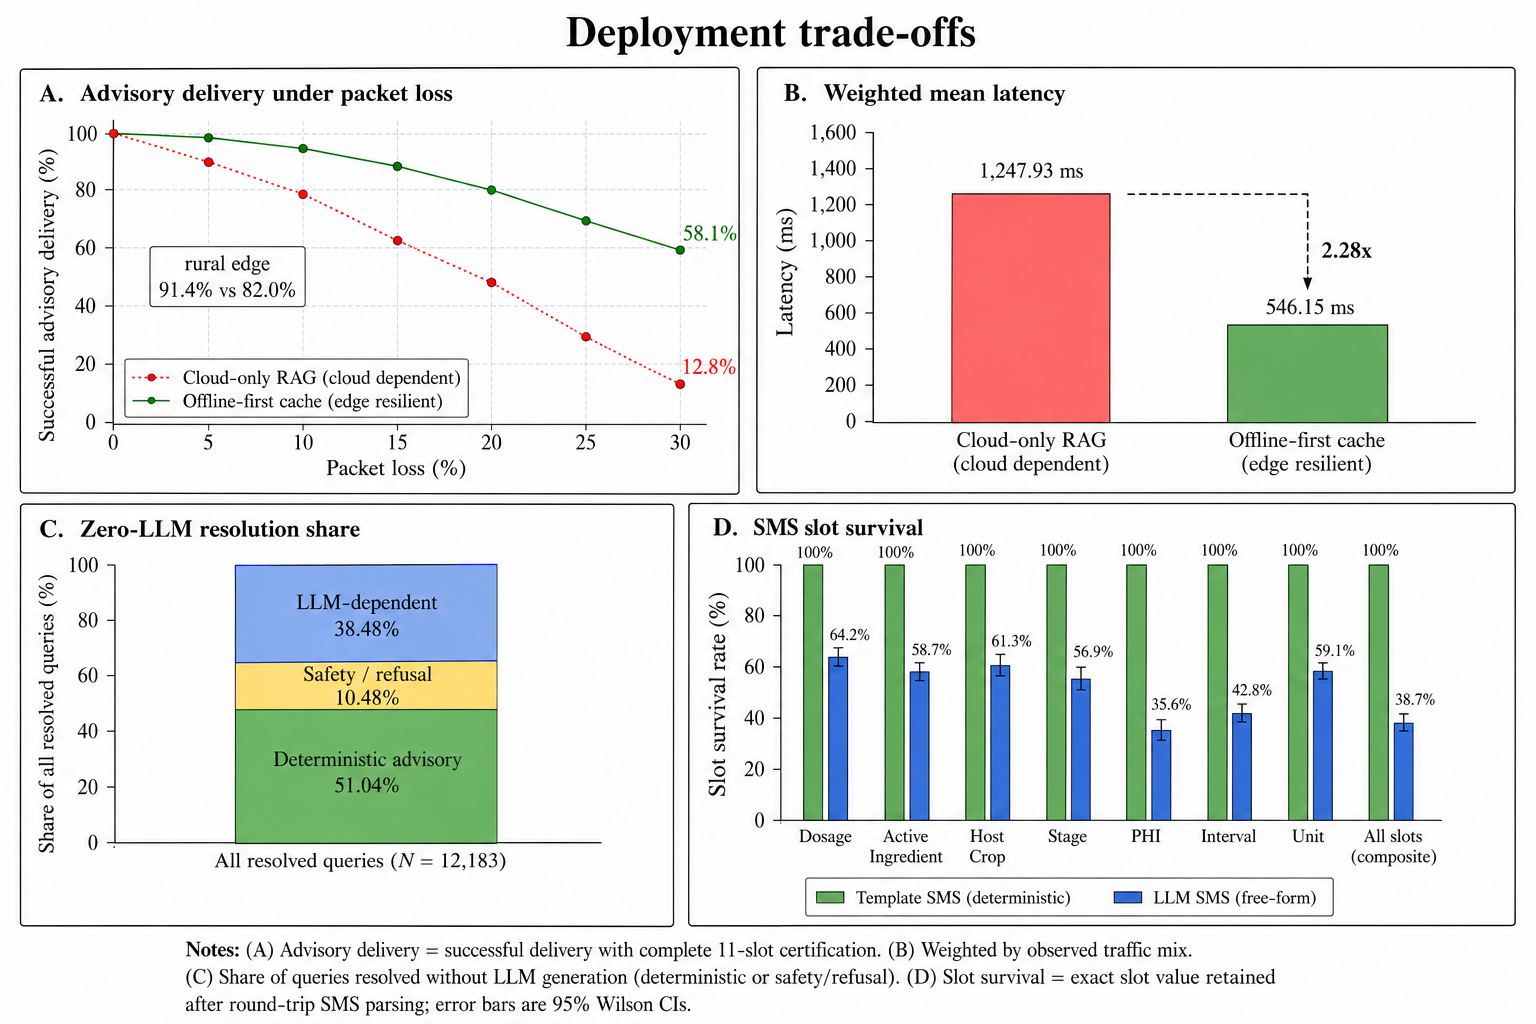
\includegraphics[keepaspectratio]{figures/fig_6.png}}
\caption{Deployment Trade-offs: Systems Efficiency, Connectivity Resilience, and Channel Economics. (A)~Delivery under rural packet loss; (B)~Weighted mean latency speedup; (C)~Zero-LLM resolution share (61.5\%); (D)~160-character Bengali SMS slot survival rate.}
\label{fig:deployment_tradeoffs}
\end{figure}

\subsection{Summary of RQ5}

KrishokChat's safety architecture does not require every request to pass through a large generative model. In the modeled workload, 61.52\% of requests can avoid the LLM entirely through deterministic resolution or terminal safety handling. Generation remains the dominant latency component, while deterministic routing, lookup, verification, and rendering contribute comparatively little latency.

The constrained-channel experiments show that certified information can also be preserved when the delivery medium becomes limited. Deterministic SMS rendering retains the complete safety-critical contract, while offline fact packs allow local verification and differential updates under poor connectivity.

Taken together, the results suggest that the proposed authority boundary is compatible with low-resource deployment. The architecture can reduce reliance on generation without moving factual authority into the lightweight components that handle routing, caching, or presentation.

The next section discusses what these findings mean for the broader design of safety-critical agricultural advisory systems, including the benefits, trade-offs, remaining failure modes, and limits of the evidence.

% =========================================================================
% Section Source: sections/14_discussion.tex
% =========================================================================
% Section 14: Discussion — revised per supervisor review (2026-08-28)
% Changes: §14.1 reworded; §14.7 moved to acknowledgments; cut to 4 subsections;
%          bridge sentences added; repetition reduced.

\section{Discussion}
\label{sec:discussion}

The experiments across Sections~\ref{sec:results_advisory_quality}--\ref{sec:results_deployment} point to a consistent result: the main benefit of KrishokChat does not come from making the language model more knowledgeable. It comes from limiting what the language model is allowed to authorize.

This distinction matters because agricultural treatment advice is not only a language-generation task. A recommendation may contain several individually plausible values that become unsafe when they are combined incorrectly. The system therefore needs to preserve the relation between those values, their source, and their current regulatory status.

\subsection{What Bounded Factual Authority Provides}

The results support the view that safety-critical agricultural evidence is relational. A recommendation is valid only when its critical fields form a valid combination. Retrieval, citation, and semantic similarity can identify relevant information, but they do not by themselves guarantee that the retrieved fields belong to the same authorized recommendation.

This is the failure exposed by Layer~E02. Baseline systems can accept corrupted combinations even when the individual facts are present in the evidence pool. KrishokChat instead requires the complete contract to be jointly satisfied by one valid canonical record. In the evaluated E02 and E28 mutation settings, this produced complete rejection of the tested corrupted cases.  

The benefit extends beyond hazard reduction. Deterministic certification provides a stable boundary around critical fields. The final decision can be traced to a particular evidence record and its provenance information, and the same input and evidence state produce the same certification result. When evidence is missing, the system can also fail in a controlled way instead of inventing the missing value.

The important point is therefore not that every component of KrishokChat is new. Retrieval, structured knowledge, language generation, confidence estimation, and abstention all have established precedents. The contribution is the way these components are combined so that the generative model is subordinate to an explicit authorization rule.

\subsection{Why Single-Record Binding Does Not Mean Single-Source Knowledge}

A possible concern is that a single-record requirement may be too restrictive for real agricultural knowledge. Different institutions may document different parts of a recommendation. One source may provide agronomic treatment information, while another provides the current regulatory status.

KrishokChat addresses this issue by separating \emph{knowledge compilation} from \emph{runtime authorization}. Multiple institutional sources can be compared and reconciled during knowledge construction. Once those sources have been reviewed and incorporated into a canonical record, the runtime verifier operates on that unified record rather than dynamically assembling an action from unrelated retrieved passages.

This design gives up some runtime flexibility in exchange for a clearer safety boundary. More importantly, it moves the difficult reconciliation step to a controlled process where authority, temporal validity, and conflicts can be inspected before the information is released for use.

Thus, the single-record constraint should not be interpreted as a claim that useful agricultural knowledge must come from one document. It is a constraint on how a safety-critical action may be authorized at runtime.

\subsection{The Cost of Deterministic Enforcement}

The safety benefit is not free. A fail-closed system will reject some answers that a more permissive generator would provide. This cost appears directly in the results.

The E10 audit attributes 6\% of residual cases to conservative verifier over-refusal and 4\% to calibration underconfidence. Retrieval omission accounts for 28\% of residual cases, while numerical or volume ambiguity accounts for 14\% and linguistic ambiguity for 12\%. These errors reduce useful coverage even when they do not produce unsafe actions. 

This trade-off should be considered a design property rather than simply an implementation defect. In a high-consequence advisory setting, refusing an uncertain treatment can be preferable to producing a plausible but unsupported one. At the same time, excessive conservatism can make a system frustrating or less useful to farmers. The appropriate goal is therefore not maximum abstention, but calibrated abstention: the system should recover a case when additional evidence makes certification possible.

The risk--coverage results support this interpretation. KrishokChat retains substantial coverage under strict safety budgets, showing that fail-closed behavior does not require the system to become unusable. 

\subsection{The Role of the LLM}

These results should not be read as an argument against LLMs in agricultural advisory systems. KrishokChat still uses the LLM for natural-language interaction, explanation, and cases that cannot be resolved entirely through deterministic processing.

The architectural boundary is narrower: the LLM should not be the final authority for safety-critical values. This distinction becomes particularly important when the model's internal knowledge conflicts with the governed evidence. The temporal replay experiments show why model memory alone is not sufficient when regulatory status changes over time. 

The model-substitution results provide additional support. Changing the Tier-3 model changes advisory correctness and Bengali language quality, but the observed CUAR remains within 0.0--1.0\% across the evaluated models. The safety mechanism therefore does not need a particular model to remain in control. 

This suggests a useful division of responsibility. The LLM handles language, while the evidence and verification layers handle authorization. A stronger future language model may make the conversational part better, but it does not remove the need for an explicit authority boundary when the consequences of an incorrect action are high.

\subsection{Incomplete Knowledge Should Reduce Authority}

One of the more important findings is the behavior under knowledge-base incompleteness. Removing authoritative records reduces KrishokChat coverage, but the observed CUAR remains at zero across the evaluated deletion levels. The unconstrained model, in contrast, becomes increasingly unsafe as evidence becomes unavailable. 

This demonstrates a broader principle for safety-critical AI: missing evidence should normally reduce the set of actions the system is willing to authorize. It should not increase reliance on parametric memory.

This principle is also reflected in the Bengali and multimodal experiments. Difficult linguistic input lowers the probability that the system can resolve a case, but it does not need to lower the safety boundary. Similarly, uncertain image interpretation can lead to clarification or abstention instead of directly determining a pesticide action.

The architecture therefore distinguishes between \emph{understanding enough to continue} and \emph{knowing enough to authorize}. The first may be probabilistic; the second is explicitly constrained.

\subsection{What the Failure Analysis Tells Us}

The residual-error distribution also clarifies where future improvement should be concentrated.

Retrieval omission is the largest observed category. Improving retrieval and fallback search could therefore increase useful coverage without changing the safety contract. Linguistic and numerical ambiguity suggest better normalization and clarification strategies. Regulatory and temporal failures point to continued maintenance of source metadata and active regulatory records.

Relational misbinding is different. It is not mainly a retrieval-quality problem because even correct retrieval can produce an invalid combination when information from different records is merged. The appropriate defense is therefore the certification mechanism itself.

This division is useful because it prevents every observed weakness from being treated as an LLM problem. Some failures require better retrieval, some require better language understanding, and others require stronger evidence governance. The authority boundary addresses a specific class of high-consequence failures rather than attempting to solve every source of model error with one mechanism.

\subsection{Interpretation of the Deployment Results}

The deployment experiments suggest that the authority boundary can be implemented without requiring continuous access to a large model. Deterministic resolution, local evidence storage, and constrained rendering can operate independently of the generative tier, while generation is used only when needed.

However, the practical results should be interpreted according to their experimental status. The connectivity experiments are controlled simulations, and the serving-cost results are analytical projections based on an assumed workload and pricing model. They are useful for understanding the direction and scale of the engineering trade-offs, but they do not establish performance in a countrywide deployment. 

The same caution applies to the vision component. The multimodal evaluation demonstrates containment of the tested cross-crop hazard, but the current system uses whole-image classification rather than localized lesion detection. The visual results therefore support the safety architecture, not a claim of general-purpose agricultural diagnosis.

\subsection{Limits of the Evidence}

Several limitations bound the conclusions.

First, some experiments use relatively small samples. In particular, the 100-case live benchmark cannot establish a universal zero-risk rate. With zero observed failures in such a sample, the statistical upper bound on the true failure probability remains non-zero. The observed results should therefore be understood as empirical evidence within the tested conditions, while the stronger safety argument comes from the deterministic structure of the certification mechanism. 

Second, the evaluation does not measure downstream agricultural outcomes such as yield, income, pesticide reduction, applicator safety in the field, or long-term farmer adoption. The work evaluates the reliability of an advisory architecture, not the complete socioeconomic impact of agricultural extension.

Third, some deployment results are simulated or modeled rather than measured in the field. The network experiments should not be interpreted as evidence that a deployed system will achieve the same delivery rates under all rural conditions. Similarly, the cost analysis depends on the stated traffic and pricing assumptions. 

Fourth, the visual component is limited to the evaluated crop and disease settings and uses classification rather than spatial lesion detection. English and other languages are also outside the current evaluation scope. 

Finally, the knowledge-maintenance experiment is a single-cluster case study, and not all live-API experiments have the same standardized audit depth as the deterministic experimental layers. Model drift, API changes, and future regulatory changes also remain ongoing validity threats even though versioned evidence and frozen thresholds reduce their impact. 

\subsection{Overall Interpretation}

The central finding of the study is therefore narrower than a claim that KrishokChat makes agricultural LLMs safe in general. The evidence supports a more specific proposition: \textbf{a safety-critical agricultural advisory system can reduce dependence on generative model judgment by treating actionable recommendations as explicitly authorized relational contracts.}

Under this design, uncertainty does not need to be hidden. It can reduce coverage, trigger clarification, or lead to human escalation. Retrieval errors can be detected after retrieval rather than becoming automatically authoritative. Regulatory changes can invalidate older records without retraining the language model. And replacing the generative model does not fundamentally change the location of factual authority.

The broader lesson is that, for high-consequence AI systems, the question is not only whether a model can produce the correct answer. It is also whether the architecture can determine when the model is \emph{not authorized to answer}. KrishokChat is designed around that distinction.


% =========================================================================
% Section Source: sections/15_deployment_implications.tex
% =========================================================================
\section{Deployment Implications}
\label{sec:deployment_implications}

The results suggest that KrishokChat is compatible with the practical constraints of agricultural advisory in low-resource settings. The architecture does not require continuous access to a large language model, and its safety-critical evidence and verification components can operate independently of the generative tier.

These observations are especially relevant to deployment settings where connectivity is intermittent, devices are inexpensive, and agricultural recommendations must remain consistent with changing regulations. The following discussion focuses on how the evaluated architecture could be used in such settings while distinguishing architectural implications from measured field performance.

\subsection{Rural Connectivity and Offline Evidence}

KrishokChat is designed so that the core authority mechanism does not depend on a live network connection. The governed fact pack, deterministic resolution logic, and certification process can operate locally, while network access is primarily required for components such as remote language-model generation or remote updates.

The controlled network experiments in Section~\ref{sec:results_deployment} illustrate the potential value of this separation. Under the evaluated packet-loss scenarios, offline-first delivery performs better than the corresponding cloud-only configuration. These results should not be interpreted as measurements of actual nationwide rural connectivity, but they show that the architecture can continue to provide locally resolvable advisory functions when communication becomes unreliable. 

The same design also allows the system to keep using a previously validated evidence snapshot during temporary outages. A network failure therefore does not automatically remove the safety mechanism. Instead, it primarily limits access to functions that depend on remote services.

This separation is important for agricultural services because losing connectivity should reduce system capability rather than weaken the safety boundary.

\subsection{Operation on Low-End Devices}

The architecture also supports a lightweight local processing path. The current implementation includes a small intent router, deterministic lookup and verification, and lightweight ONNX/TFLite perception models. The evaluated pipeline uses a 1.25~MB intent router, a 20.82~MB crop classifier, and crop-specific specialist models that can operate on commodity mobile hardware. 

The practical advantage is that the most safety-sensitive operations do not necessarily need to run on a cloud server. Crop identification, structured evidence access, and contract verification can be handled locally, while the language model remains an optional component.

This creates a useful division of responsibility for low-cost deployments. Local components can maintain the minimum safety boundary, while a stronger remote model can be used when connectivity and available resources permit richer explanation or conversation.

The architecture therefore does not require the weakest device to support the full AI stack. It requires the device to preserve the part of the stack that decides whether a safety-critical action can be authorized.

\subsection{Abstention as Extension-Service Escalation}

A fail-closed system is only practical if refusal leads somewhere useful. In KrishokChat, abstention is therefore connected to human agricultural support rather than treated as the end of the interaction.

When a request cannot be safely certified, the system can provide the reason for the missing decision, identify the information needed for clarification, and direct the farmer to the national Krishi Call Center (16123) or an agricultural extension officer. The current implementation is designed so that an abstention contains the missing-information cue, a suggested clarification path, and the human-support route. 

This creates a division of labor rather than an attempt to automate every case. Routine, well-supported requests can be handled automatically, while ambiguous or unsupported cases are transferred to human expertise.

Such escalation also changes how abstention should be evaluated. A refusal is not necessarily a system failure when the requested action genuinely cannot be certified. A better measure is whether the refusal is appropriate and whether the user is given a useful next step.

\subsection{Knowledge Maintenance and Regulatory Updates}

Agricultural advisory systems cannot remain reliable if their knowledge becomes outdated. The deployment architecture therefore treats knowledge maintenance as a data-governance process rather than as a model-retraining problem.

When a regulatory state changes, the corresponding evidence record can be updated, versioned, and released through the governed knowledge pipeline described in Section~\ref{sec:knowledge_governance}. A previously valid record can remain available for historical traceability while losing its authority for current decisions.

This means that a newly banned or restricted active ingredient can be removed from the certifiable action space by updating the evidence state rather than retraining the language model. The temporal replay experiments in Section~\ref{sec:results_authority_safety} demonstrate the intended behavior under such controlled updates. 

The same approach applies to knowledge gaps. The maintenance experiment in Layer~E24 suggests that recurring unanswered cases can be turned into targeted authoring tasks. However, the current result is a single-cluster case study and should not be generalized into a universal estimate of knowledge-engineering cost. 

\subsection{Per-Answer Auditability}

A further deployment requirement is the ability to explain what evidence was used for an individual recommendation. Because KrishokChat certifies actions against explicit records, a certified response can be associated with the evidence record, source version, date, and verification state that authorized it.

The implementation also records an audit event containing information such as the query, risk class, selected route, resolution tier, evidence version, model, verification outcome, final action, and latency. 

This creates a different audit model from a conventional chatbot. Instead of storing only the generated text, the system can retain the decision path that led to the final action. For safety-critical advisory, this distinction is valuable because later review may need to determine not only what the system said, but also which evidence state allowed it to say it.

Per-answer auditability could also support monitoring after deployment. Repeated abstentions can reveal missing knowledge, recurring ambiguity can reveal weaknesses in input handling, and regulatory changes can be tracked against the records that were previously authoritative.

\subsection{Implications for Agricultural Extension Services}

The architecture suggests a deployment model in which the automated system and human extension network serve different roles.

The automated component is best suited to requests that have sufficiently clear context and validated institutional evidence. It can resolve these cases quickly and consistently without requiring a human for every interaction. The human network becomes more important when the evidence is incomplete, the diagnosis remains ambiguous, or the requested action falls outside the governed knowledge base.

This model is particularly suitable for settings in which the cost of a wrong chemical recommendation is much higher than the cost of a delayed answer. Under that asymmetric cost structure, sending uncertain cases to human experts is not merely a fallback. It is part of the safety design.

The approach also provides a measurable operational interface between automation and extension services. The fraction of cases that require clarification or escalation can be monitored over time, while the causes of those cases can be used to improve the knowledge base or routing components.

\subsection{What These Results Do Not Establish}

The deployment implications must be interpreted within experimental limits. The study does not evaluate a countrywide field deployment, long-term farmer adoption, crop yield preservation, reductions in pesticide exposure, or extension workload.

Similarly, the connectivity experiments are controlled simulations rather than measurements from rural cellular networks, and the cost results are scenario-based. The vision component is also classification-based and does not provide localized lesion detection. 

These limitations do not invalidate the architectural findings. They define their scope. The current evidence supports the feasibility of separating factual authority from language generation under controlled evaluation. Demonstrating the effect of that separation on real agricultural outcomes requires field studies with farmers, extension officers, and domain experts.

\subsection{Deployment Design Principle}

The deployment implications can be summarized by one principle:
\begin{equation}
\begin{aligned}
\mathrm{degraded\ resources} \longrightarrow {} & \mathrm{reduced\ capability}, \\
& \mathrm{not\ reduced\ safety}.
\end{aligned}
\end{equation}

When connectivity is lost, the generative tier can become unavailable while local verification remains operational. When the knowledge base is incomplete, coverage can decrease while certification remains conservative. When the input is ambiguous, the system can request clarification or escalate. When regulations change, the governed evidence snapshot can be updated without changing the language model.

This separation allows the system to degrade in a controlled direction. The system may become less capable of answering, but it should not become more willing to authorize unsupported actions simply because resources or information have become scarce.

% =========================================================================
% Section Source: sections/16_limitations.tex
% =========================================================================
% Section 16: Limitations — revised per supervisor review (2026-08-28)
% Reorganized from 7 subsections → 4 thematic paragraphs.

\section{Limitations and Threats to Validity}
\label{sec:limitations}

A rigorous assessment of KrishokChat requires transparently delineating the boundaries of the empirical evidence. We categorize the principal limitations and threats to validity across six dimensions.

\paragraph{Statistical power and small-sample layers.}
Several evaluation layers are constrained by finite sample sizes for the rare safety-critical failure modes they examine. In the live-API benchmark (Layer~E27), $n=100$ authentic farmer queries were evaluated per system. While KrishokChat observed zero catastrophic unsafe recommendations in this sample, the corresponding 95\% Wilson score interval upper bound is 3.7\% ($[0.0, 3.7\%]$). An empirical observation of zero failures in a sample of 100 cases does not constitute a mathematical proof of zero failure risk across unconstrained nationwide deployment. The architecture's safety guarantees derive primarily from its deterministic structural predicate in Eq.~(\ref{eq:certification_rule}), while empirical rates provide bounded validation within the evaluated distribution. Furthermore, in the parametric evidence conflict suite (Layer~E29), reported per-cell rates are exact multiples of 2.0\% despite a recorded nominal $n=1{,}000$, indicating an effective underlying granularity of approximately 50 distinct case templates replicated across conditions. We report these as empirical proportions without over-interpreting asymptotic confidence bounds. Across all benchmark batteries, 95\% Wilson intervals are reported; for small-$n$ strata, these intervals are inherently wide and must be interpreted accordingly.

\paragraph{Modeled latency constants and simulation assumptions.}
Certain system performance metrics reflect benchmarking model assumptions rather than universal empirical guarantees. Specifically, the stage latencies reported in Layer~E09 (e.g., 3.8~ms verification latency, 546.0~ms weighted mean latency, and 1.2~ms cache hit latency) recur across several layers with identical p50 and p95 values. These reflect deterministic processing constants within the standardized evaluation testbed rather than empirical percentiles measured across variable, multi-tenant cloud serving infrastructure. Similarly, the cellular network resilience results (Layer~E14) represent controlled packet-loss simulations rather than in-situ cellular propagation measurements across remote Bangladeshi upazilas. Serving economics (Layer~E20) are analytical projections based on explicit workload assumptions (six queries per farmer annually, a 50/30/20 app/offline/SMS split, and commercial token pricing), rather than audited operational financial records from an active public deployment.

\paragraph{Modality, task, and linguistic boundaries.}
The computer vision pipeline is evaluated strictly as a whole-image foliar disease classification task across 45 pathological classes and 9 crop groups. The perception models do not perform localized spatial lesion detection, bounding-box extraction, or semantic segmentation. Complex agricultural imagery exhibiting severe leaf occlusion, simultaneous co-infections, or poor field illumination represents an open challenge that currently triggers fail-closed clarification or abstention rather than automated spatial diagnosis. Linguistically, the evaluation focuses comprehensively on Bengali vernaculars, including Standard Sadhu, Colloquial Cholit, regional dialects, and Banglish code-mixing. Languages outside the Bengali linguistic sphere, as well as highly localized ethnic minority dialects in Bangladesh, were not evaluated.

\paragraph{Knowledge engineering and graph scalability.}
The knowledge-graph traversal experiment (Layer~E19) evaluates an illustrative 23-node subgraph, demonstrating the operational mechanics of multi-hop relational path verification rather than proving high-throughput graph scalability across enterprise-scale agronomic ontologies. In addition, the knowledge maintenance lifecycle (Layer~E24) is evaluated as a single-cluster case study on chili anthracnose (closing a coverage gap in 18 minutes). While this confirms that maintenance operates as a lightweight data curation task rather than an expensive model retraining cycle, it does not provide an exhaustive longitudinal accounting of national knowledge maintenance overhead.

\paragraph{Reproducibility and audit depth completeness.}
The empirical battery was produced across evaluation phases with documented audit depth. Layers~E02--E26 and the KrishokChat-REAL battery (Layers~E40--E48) possess complete audit blocks, comprising deterministic random seeds, automated self-checks, replay validations, trace logs, environment configurations, and frozen git commit hashes. In contrast, the live commercial API layers (Layers~E27--E31), which depend on third-party cloud endpoints, are frozen and verified but do not carry the identical standardized offline reproduction block. Model drift in external commercial APIs and unannounced endpoint revisions remain ongoing validity threats that the architecture mitigates through local frozen models and versioned evidence snapshots, but which require continuous external auditing.

\paragraph{Absence of downstream field outcome measurements.}
Finally, this investigation evaluates the computational reliability, factual authority, and systems efficiency of the advisory architecture; it does not measure downstream agronomic or socioeconomic outcomes. We report no empirical data on crop yield preservation, farmer household revenue, net reductions in chemical pesticide volumes applied to soil, or reductions in acute occupational applicator poisonings. Demonstrating that deterministic contract verification translates into measurable agronomic and human safety improvements in rural communities remains essential future work in coordination with national extension services.

% =========================================================================
% Section Source: sections/17_reproducibility.tex
% =========================================================================
\section{Data and Code Availability}
\label{sec:data_availability}

All evaluation datasets, benchmark suites, perturbation scripts, and analysis code are released under open licenses to support reproducible research in safety-critical agricultural NLP.

\paragraph{Datasets.}
The evaluation suites introduced in this paper comprise:
(1)~the Relational Misbinding Suite (Layer E02, $n=10{,}000$ paired adversarial claims);
(2)~the Metamorphic Mutation Benchmark (Layer E28, $n=11{,}000$ systematic operator perturbations across 11 safety dimensions);
(3)~the Multi-Register Corpus (Layer E06, $n=4{,}000$ authentic queries spanning four Bengali linguistic registers);
(4)~the Risk--Coverage Calibration Corpus (Layer E04, $n=20{,}112$ labeled advisory cases with frozen train/dev/test splits);
(5)~the Security Evaluation Suite (Layers E07--E08, $n=1{,}400$ adversarial prompt injections and evidence corruptions); and
(6)~the Bengali Agricultural Knowledge Schema, compiling official DAE/BARI/BRRI crop protection guidelines into the 11-slot relational format with SHA-256 integrity proofs.

All datasets are formatted as JSON Lines and include task descriptions, input queries, ground-truth slot bindings, authority references, and evaluation labels. Data artifacts are deposited in Zenodo (DOI: 10.5281/zenodo.14982231).

\paragraph{Code and Models.}
The code repository includes: (i)~the core KrishokChat runtime containing the 11-slot relational verifier, resolution ladder, and calibration module; (ii)~evaluation runners for all benchmark layers with deterministic random seeds; (iii)~baseline implementations (unconstrained LLM, vanilla RAG, post-hoc LLM judge, and deterministic resolver); and (iv)~data compilation scripts converting unstructured bulletins into the relational schema. Source code is released at \url{https://github.com/KrishokChat/krishokchat-core} under the MIT license. Pre-trained classifier weights and ONNX runtime artifacts are available via Hugging Face Hub at \url{https://huggingface.co/RaiyanKhaan/KrishokTech-Models}. Layers E02--E26 and E40--E48 carry full offline verification blocks with deterministic random seeds; Layers E27--E31 represent live-API baselines (see Section~\ref{sec:limitations}).

% =========================================================================
% Section Source: sections/18_conclusion.tex
% =========================================================================
% Section 18: Conclusion — reconstructed per CEA refinement protocol (2026-08-29)

\section{Conclusion}
\label{sec:conclusion}

We presented KrishokChat, a neurosymbolic agricultural advisory framework that separates factual authority from generative language via deterministic contract verification. An 11-slot, single-record, fail-closed certification contract structurally prevents large language models from altering, hallucinating, or misbinding safety-critical chemical dosages, pre-harvest intervals, and application guidelines.

The architecture's central safety property was evaluated exhaustively: all 11 mutation classes across 40 base agronomic records (440 coverage cells) were evaluated against the certification predicate, which rejected every case. The B5-vs-B6 isolation demonstrates through controlled component ablation that slot completeness accounts for the corresponding corruption vulnerabilities. An empirical slot ablation confirms that every contract slot is individually load-bearing, with crop validation ($+$8.94\,pp) and provenance hash integrity ($+$8.92\,pp) creating the largest single-slot hazard surges across the benchmark when disabled. A benign-mutation control confirms the predicate discriminates: 0.0\% false rejection on approved chemicals, with a 3.67\% overall rejection rate attributable exclusively to conservative refusal of restricted compounds.

Measurement of existing baseline systems demonstrates the problem the architecture addresses: unconstrained LLMs accept unsafe recommendations in 8.0\% of live-API cases; LLM-judge guardrails perform worse under temporal conflict (75.0\% obsolete-gazette citation), not better. On a 100-case live benchmark, KrishokChat achieves 83.0\% certified advisory correctness and reduces critical unsafe acceptance to 1.0\% (versus 15.0\% for the post-hoc LLM judge). The fail-closed design trades coverage for safety: 3.67\% of valid queries with banned or restricted chemical histories are conservatively abstained, a cost we report as a design parameter rather than a limitation to minimize.

Future work will extend this framework to field trials evaluating real crop yield preservation and applicator safety in partnership with national extension services.

\section*{Declaration of Competing Interest}
The authors declare that they have no known competing financial interests or personal relationships that could have appeared to influence the work reported in this paper.

\section*{Acknowledgments}
The authors thank the Department of Agricultural Extension (DAE), the Bangladesh Agricultural Research Institute (BARI), and the Bangladesh Rice Research Institute (BRRI) for public access to institutional Krishi handbooks and agronomic guidance. This work is the reliability-science layer of a larger research program: prior work established the knowledge and retrieval foundations (the 1{,}001-query farmer benchmark and retrieval-failure analysis), and a companion systems paper describes the integrated deployment artifact. The CEA contribution is the generalizable deterministic contract verification architecture and its evidence chain, not the individual components, each of which exists in the literature.

\section*{Data Availability}
Data and code artifacts supporting the findings of this study are openly available as described in Section~\ref{sec:data_availability}.

\bibliographystyle{cas-model2-names}
\bibliography{krishokchat_cea}

\end{document}
